\chapter{A Novel Implementation of the \glsentryshort{lartpc} Technology}
\label{chap:ac}


\section{First Results from the \AC{} Pixel Demonstrator}
\label{sec:ac_viper}

This chapter describes the results obtained from the first pixelated \lartpc{} prototype for the \AC{} project (see Chapter~\ref{sec:ac_argoncube}).
While many of the individual systems, such as the high-voltage system, light and charge readout, have been described in previous chapters, a short overview of the implementation is given here.


\subsection{Pixel \glsentryshort{pcb} Design}
\label{sec:ac_viper_pcb}
 
The pixelated anode plane, shown in Figure~\ref{fig:viper_pixies}, was produced as a conventional \gls{pcb}. 
The pixelated area is \SI{100}{\milli\metre} across, the pixels are formed of \SI{900}{\micro\metre} vias with a pitch of \SI{2.54}{\milli\metre}.
An inductive focusing grid surrounds the pixels, it is made from \SI{152.4}{\micro\metre} copper traces split into 28 regions.
There are \num{6 x 6} pixels per region, giving a total of 1008 pixels. 

\begin{figure}[htb]
	\centering
	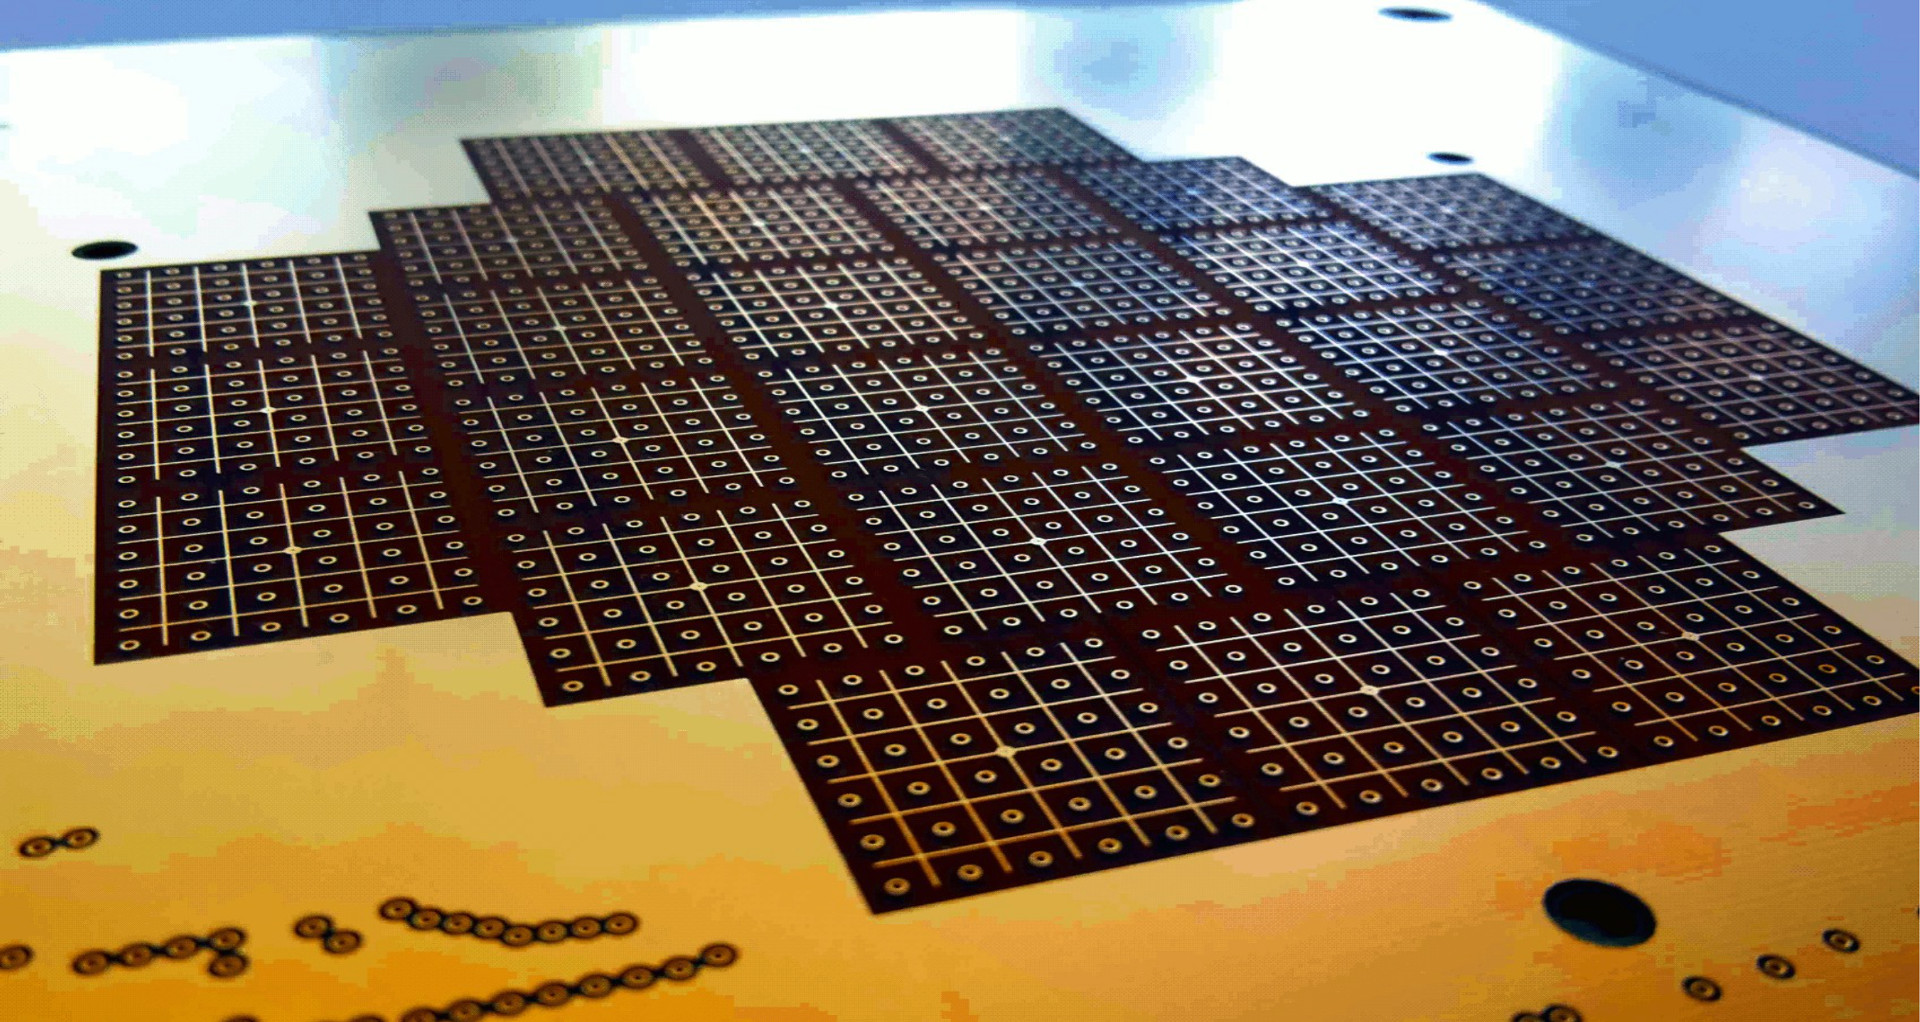
\includegraphics[width=0.65\linewidth]{viper/pixies}
	\caption{Initial (July 2016) pixelated anode \gls{pcb}. The pixelated readout area is \SI{100}{\milli\metre} in diameter.
	Each charge collection pixel is a \SI{900}{\micro\metre}, at a pitch of \SI{2.54}{\milli\metre}, inductive focusing grids formed of \SI{152.4}{\micro\metre} copper traces surround the pixels.
	There are 28 inductive focusing grids with 36 pixels per region, a total of 1008 pixels.}
	\label{fig:viper_pixies}
\end{figure}

Vias were used for pixels instead of pads in order to minimise capacitance.
As detailed in Section~\ref{sec:studies_electronics}, it is important that capacitance is minimised when amplifying charge.
To further minimise parasitic capacitance, the \gls{pcb} design was optimised by removing unnecessary ground planes, routing signal tracks outside necessary ground planes, and increasing the thickness of the \gls{pcb} to \SI{3.5}{\milli\metre} from an initial \SI{1.75}{\milli\metre}. 
The resulting capacitance at each pixel is $\approx \SI{50}{\pico\farad}$.

The pixels are directly connected to the preamplifiers while the inductive focusing grids are decoupled via \SI{10}{\nano\farad} capacitors.
Additionally, the bias voltage is filtered at the input by another \SI{10}{\nano\farad} and \SI{10}{\mega\ohm}.
The full schematic of the bias circuit is depicted in Figure~\ref{fig:viper_pcb_schematic}.

\begin{figure}[htb]
	\centering
	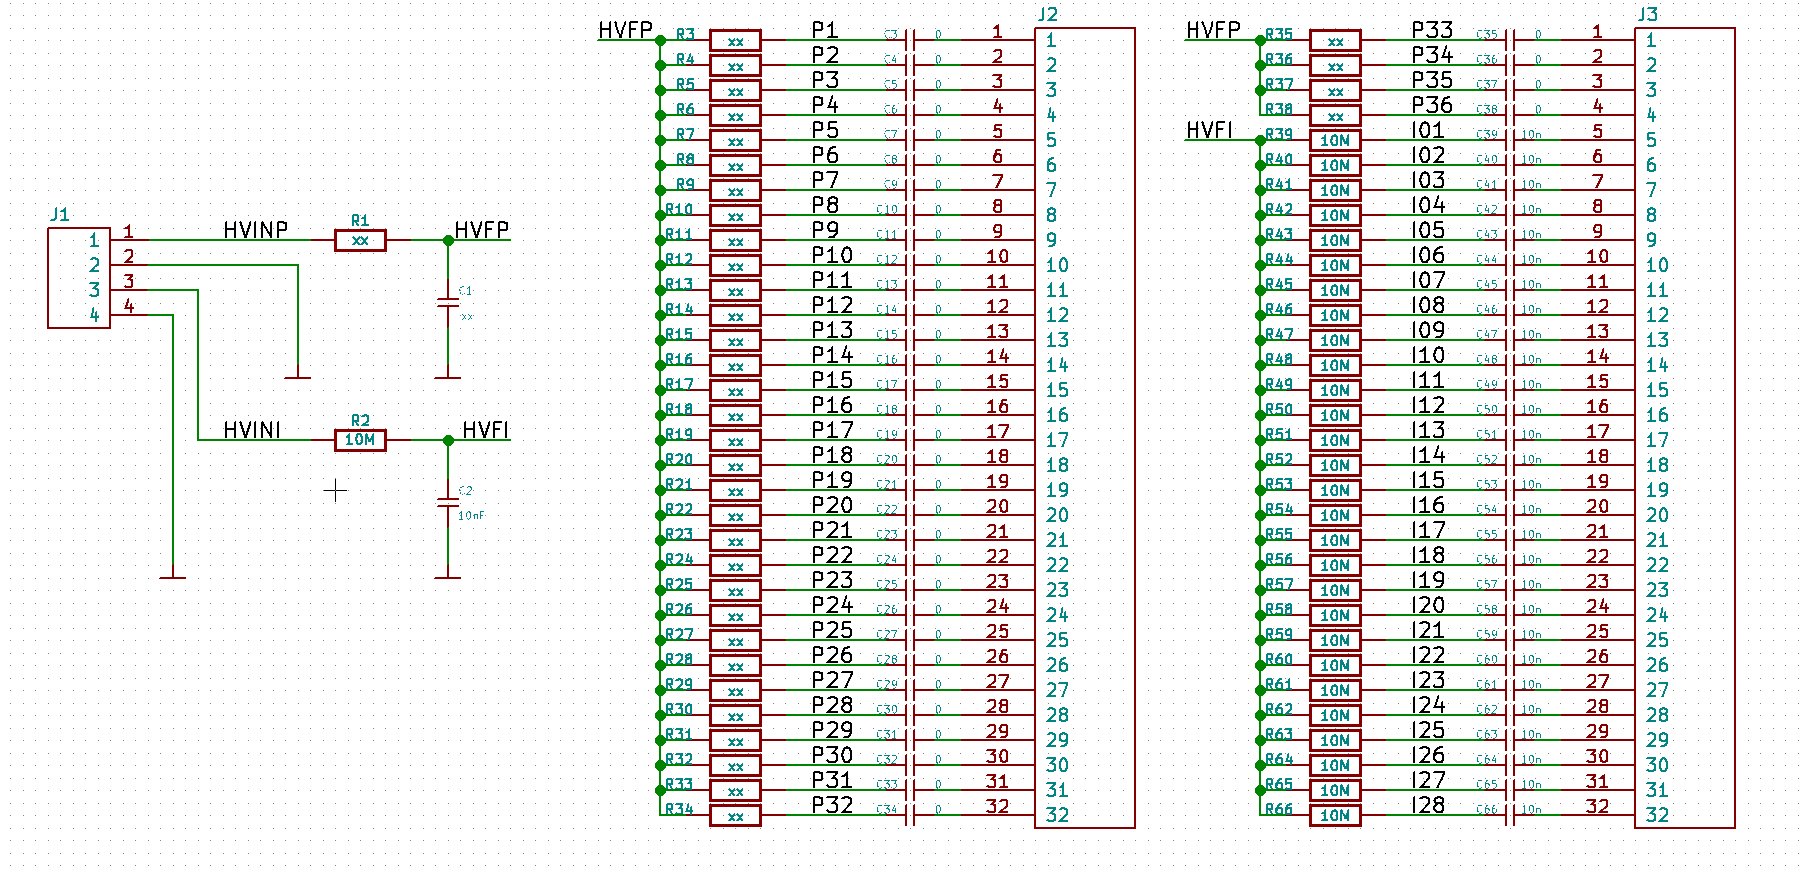
\includegraphics[width=\textwidth]{viper/pixel_pcb_schematic}
	\caption{Schematic of the bias circuit for the \AC{} pixel demonstrator \gls{pcb}.
	On the left, the pinheader connected to the bias \gls{hv} power suplly is shown. In the middle and on the right are the connections to the pixels and inductive \gls{roi} grids.
	The connections to the preamplifier inputs are located at the positions of numbers P1--P36 (pixels) and I1--I28 (\glspl{roi}).
	For simplicity and universality, the same circuit was used for both pixels and \glspl{roi} eventhough for the measurements described in this work, only the inductive \gls{roi} grids were biased.
	Therefore, the \glspl{roi} are connected as depicted (R2 and R39--R66, C2 and C39--C66).
	As the pixels need not be biased, they are directly connected to the preamplifiers by leaving R3--R38 unpopulated and replacing C3--C38 by \SI{0}{\ohm} resistors.
	Additionally, R1 is \SI{0}{\ohm} and C1 unpopulated, and by connecting pin 1 of J1 to ground, all unused \gls{pcb} traces are grounded.}
	\label{fig:viper_pcb_schematic}
\end{figure}

The bias on the inductive focusing grids had to be sufficient to allow full charge transparency (all charge collected by the pixels), yet low enough to minimise any risk of damaging the cold coupling capacitors.
It was increased incrementally until transparency was observed at \SI{300}{\volt}. 
Simulation suggest this was only \SI{95}{\percent} transparency, with \SI{100}{\percent} at \SI{350}{\volt} (see Figure~\ref{fig:viper_transparency}).
The simulation available at the time of the measurement contained a bug resulting in an underestimation of the bias voltage required for full transparency.
During measurements, the bug became apparent and full transparency had to be estimated by looking at live data from the detector.
Due to the limited accuracy of this method, measurements were not taken up to the bias voltage for full transparency suggested by the (corrected) simulation.~\cite{francypants}

\begin{figure}[htb]
	\centering
	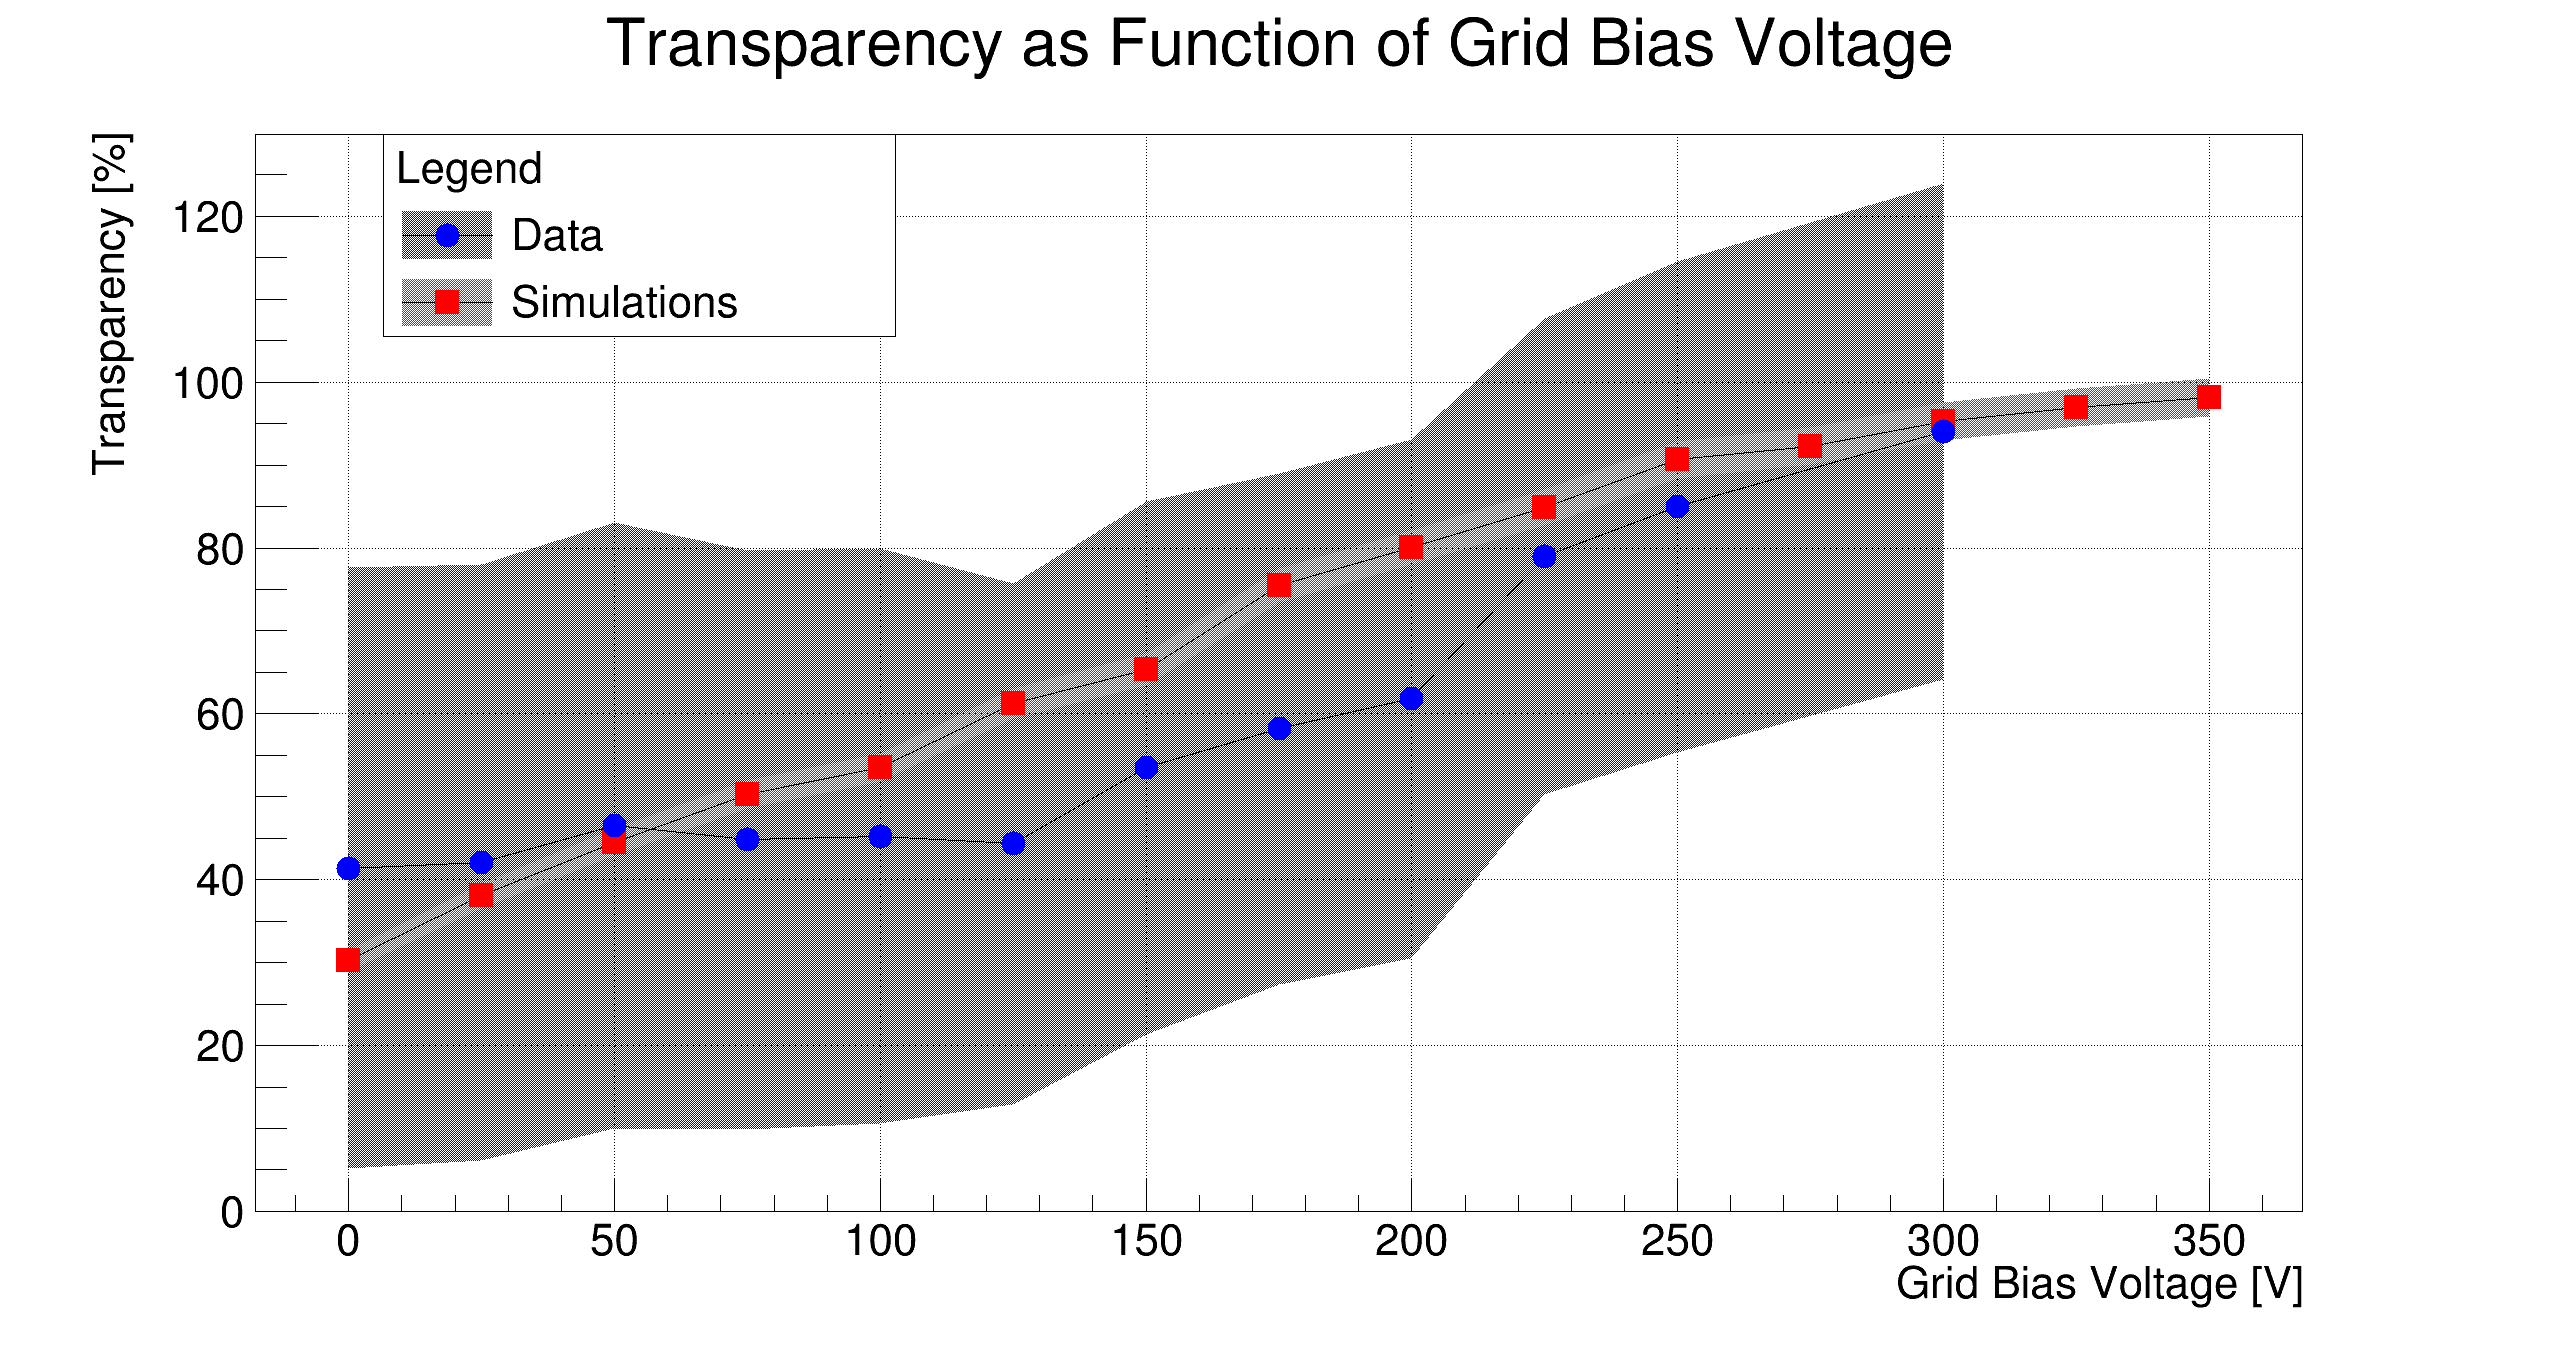
\includegraphics[width=\textwidth]{viper/transparency}
	\caption{Measured and simulated transparency versus bias voltage of the \AC{} pixel demonstrator.
	The simulation available at the time of the measurement contained a bug resulting in an underestimation of the bias voltage required for full transparency.
	During measurements, the bug became apparent and full transparency had to be estimated by looking at live data from the detector.
	Due to the limited accuracy of this method, measurements were not taken up to the bias voltage for full transparency suggested by the (corrected) simulation.~\cite{francypants}}
	\label{fig:viper_transparency}
\end{figure}


\subsection{\glsentryshort{tpc}}
\label{sec:ac_viper_tpc}

The pixel demonstration \gls{tpc}, shown in Figures~\ref{fig:viper_cad}~and~\ref{fig:viper_v1per}, is cylindrical with an inner diameter of \SI{101}{\milli\metre} and a \SI{590}{\milli\metre} drift length. 
The \gls{tpc} operated with a drift field of \SI{1}{\kilo\volt\per\centi\metre}, corresponding to a total drift time of \SI{281}{\micro\second} at \SI{2.1}{\milli\metre\per\micro\second}.~\cite{protoLASER}

\begin{figure}[htb]
	\centering
	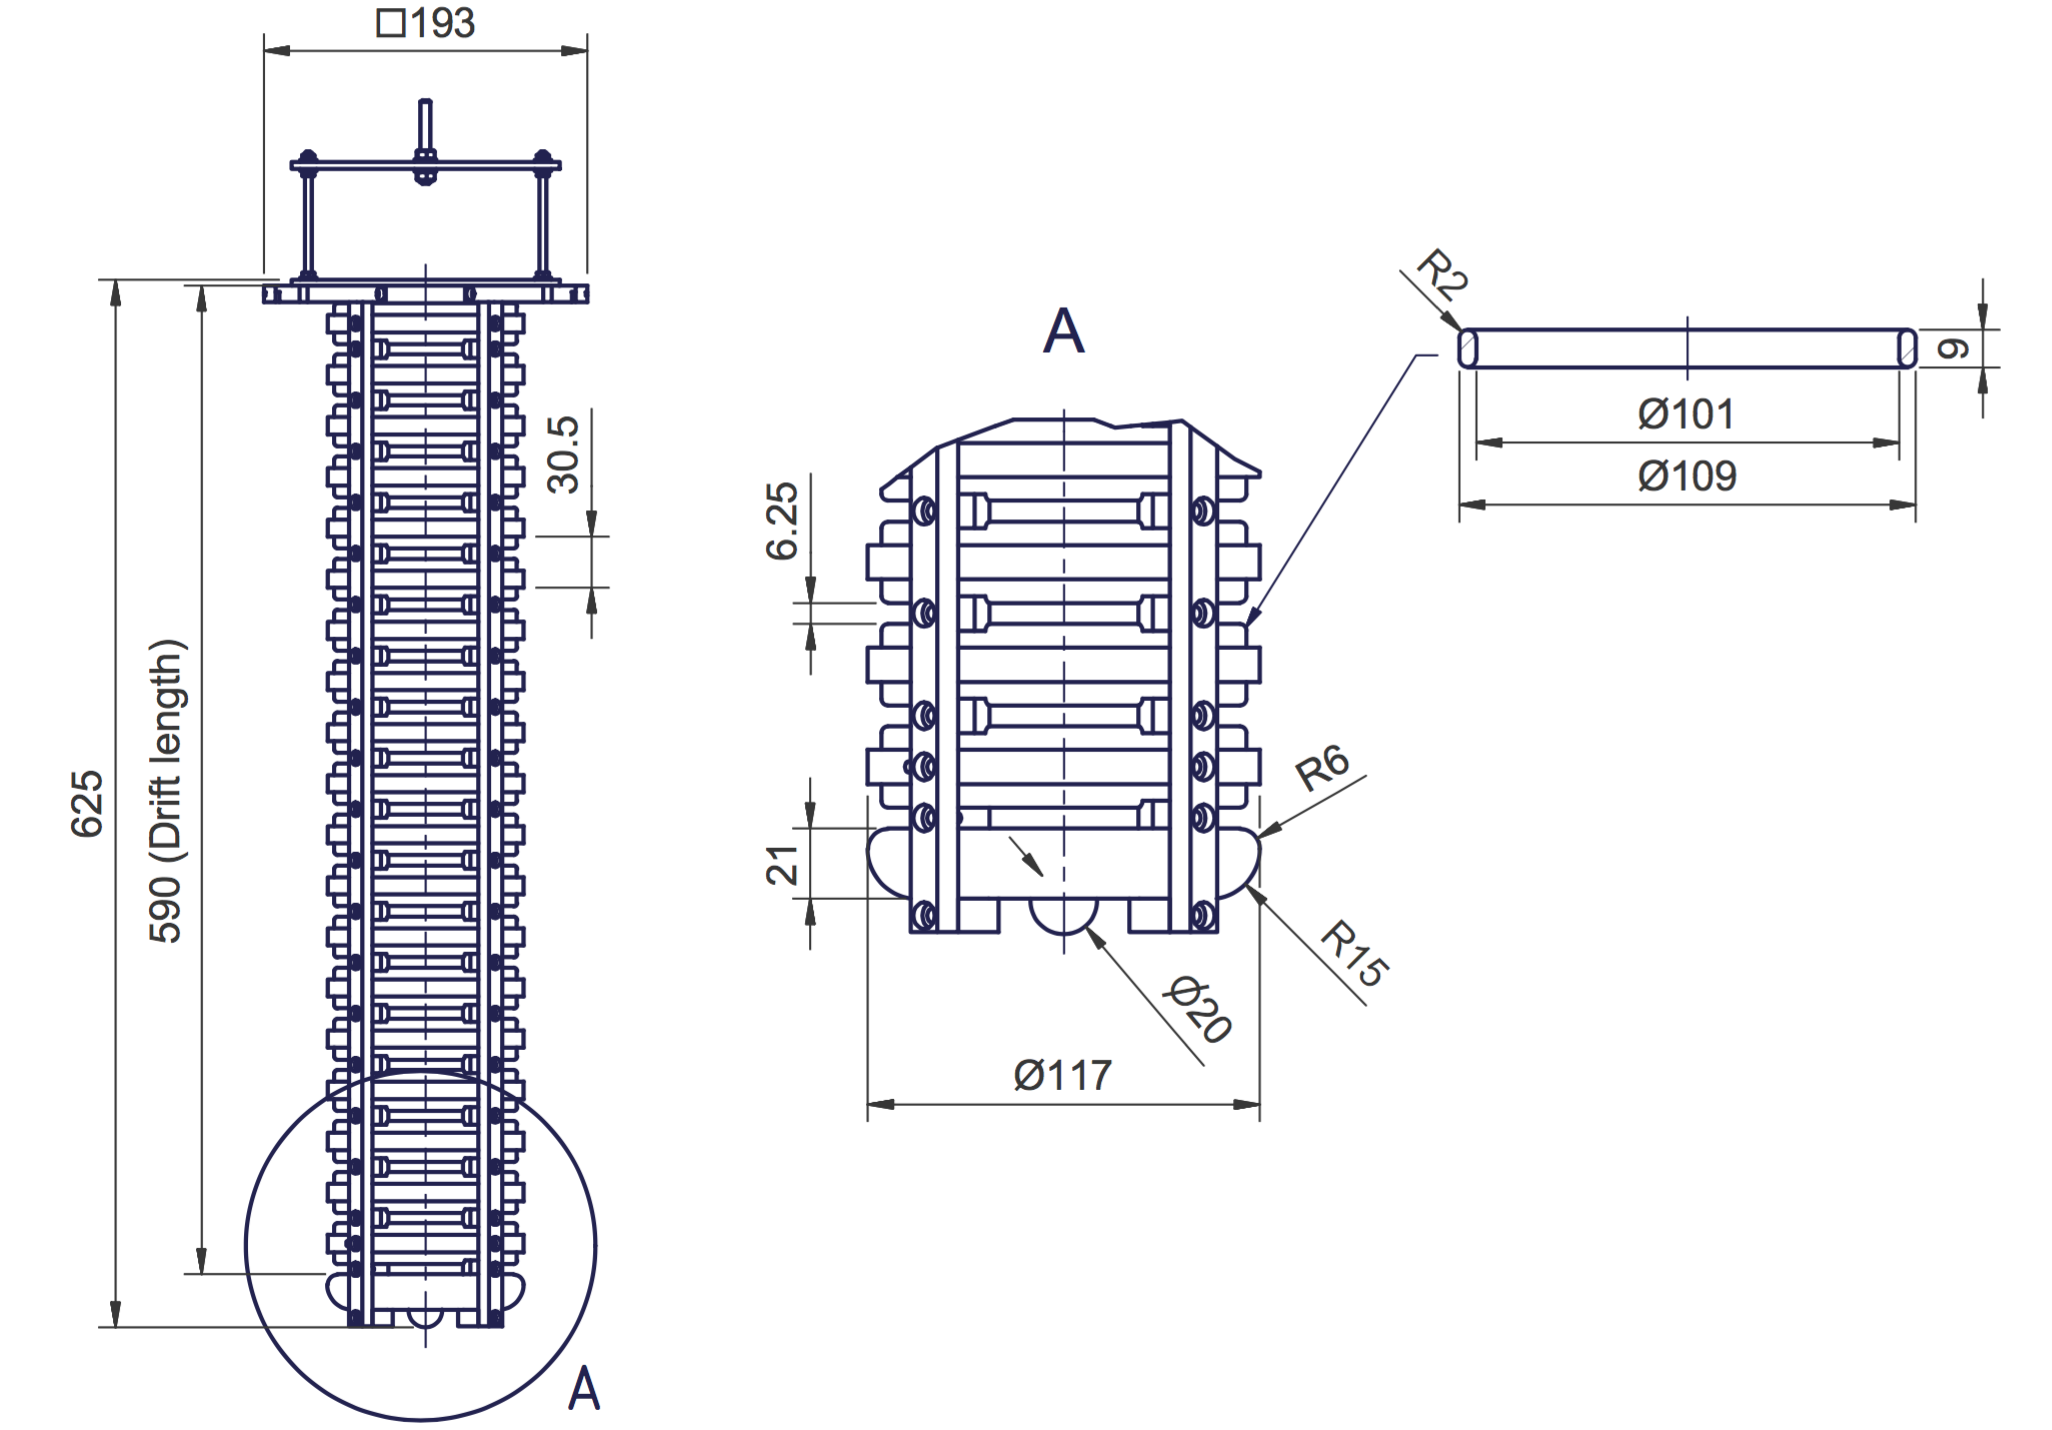
\includegraphics[width=0.9\linewidth]{viper/tpc_cad}
	\caption{\small Engineering drawing of the pixel demonstration \gls{tpc}; \SI{590}{\milli\metre} drift length; \SI{6.25}{\milli\metre} field cage spacing; \SI{101}{\milli\metre} internal diameter.}
	\label{fig:viper_cad}
\end{figure}
 
The field-cage consists of aluminium rings supported by clear acrylic rings, with a cathode formed of a brass disc. 
The dimensions of the field-cage and cathode are shown in Figure~\ref{fig:viper_cad}.
Alternating acrylic rings are split, to allow for the circulation of purified \lar{} within the \gls{tpc} volume.
Four square section PolyAmide-Imide (PAI) uprights support the cathode and field cage, with PolyEther Ether Ketone (PEEK) screws fixing the pillars to the acrylic rings.
The four PAI uprights connect to a PAI frame which supports the anode plane and the light readout \glspl{sipm}, see Figure~\ref{fig:viper_v1per}.   

The resistive divider consists of a chain of \SI{100}{\mega\ohm} Vishay Rox metal oxide resistors (ROX100100MFKEL).
Each resistor is soldered to its neighbour, and fixed to the field cage at each joint with an M3 screw.   

\begin{figure}[htb]
	\centering
	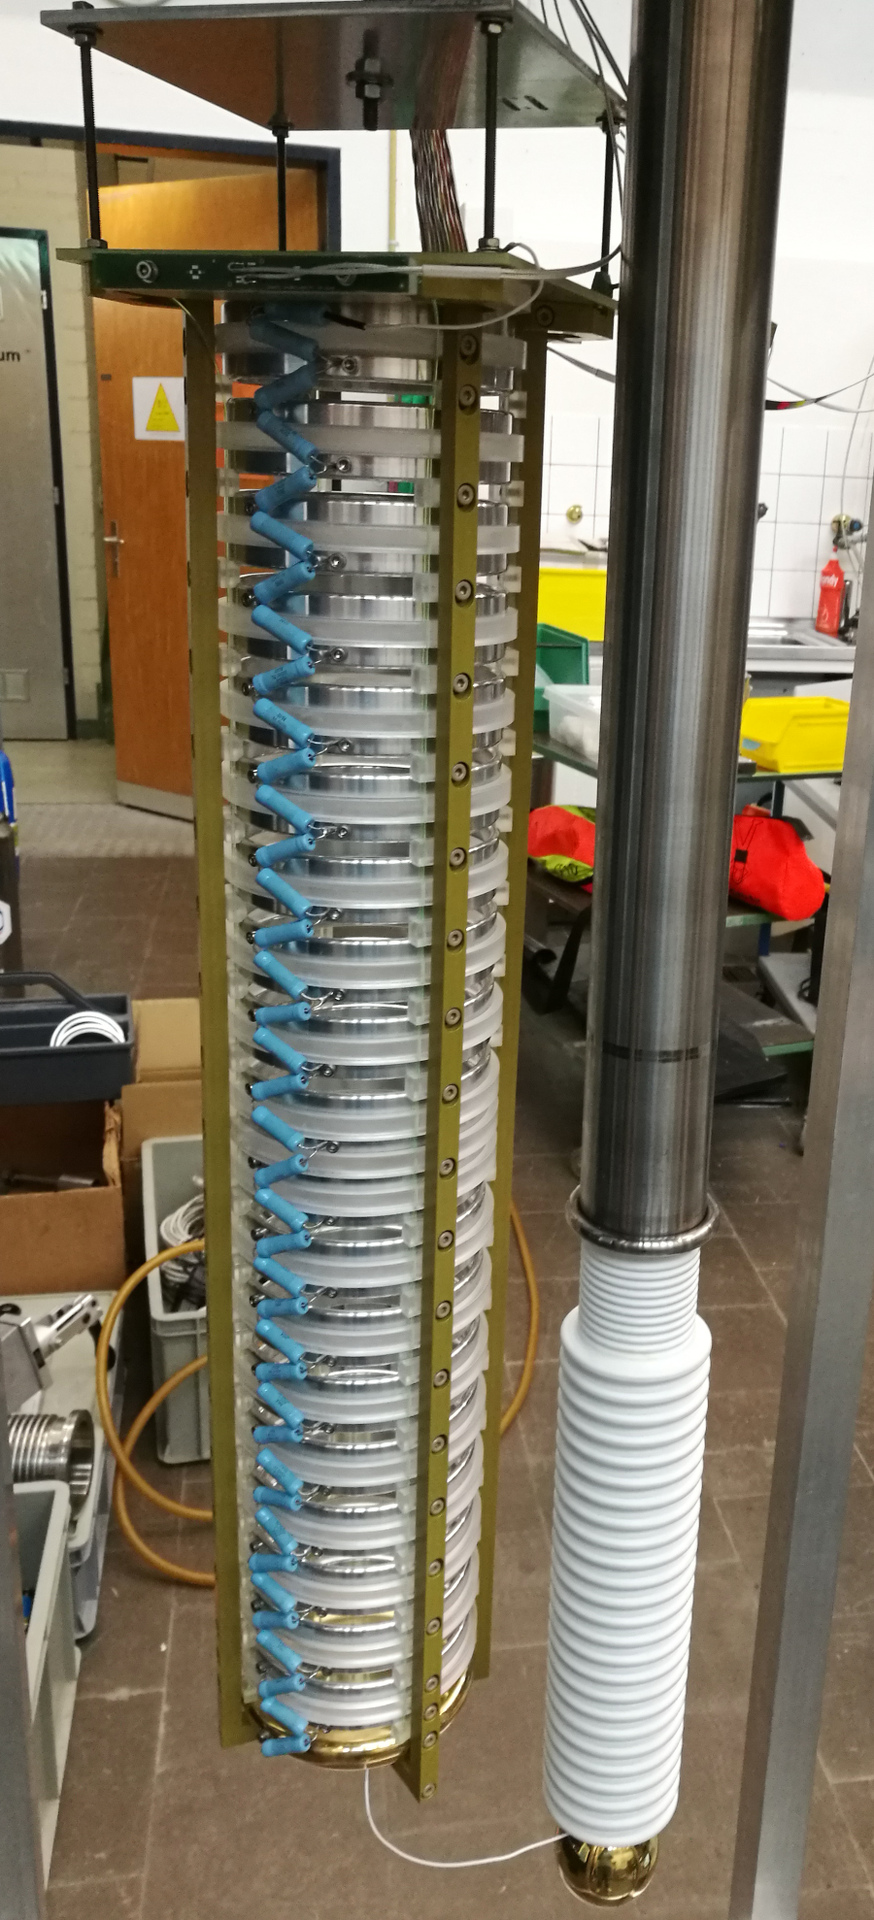
\includegraphics[width=0.26\linewidth]{viper/viper_original}
	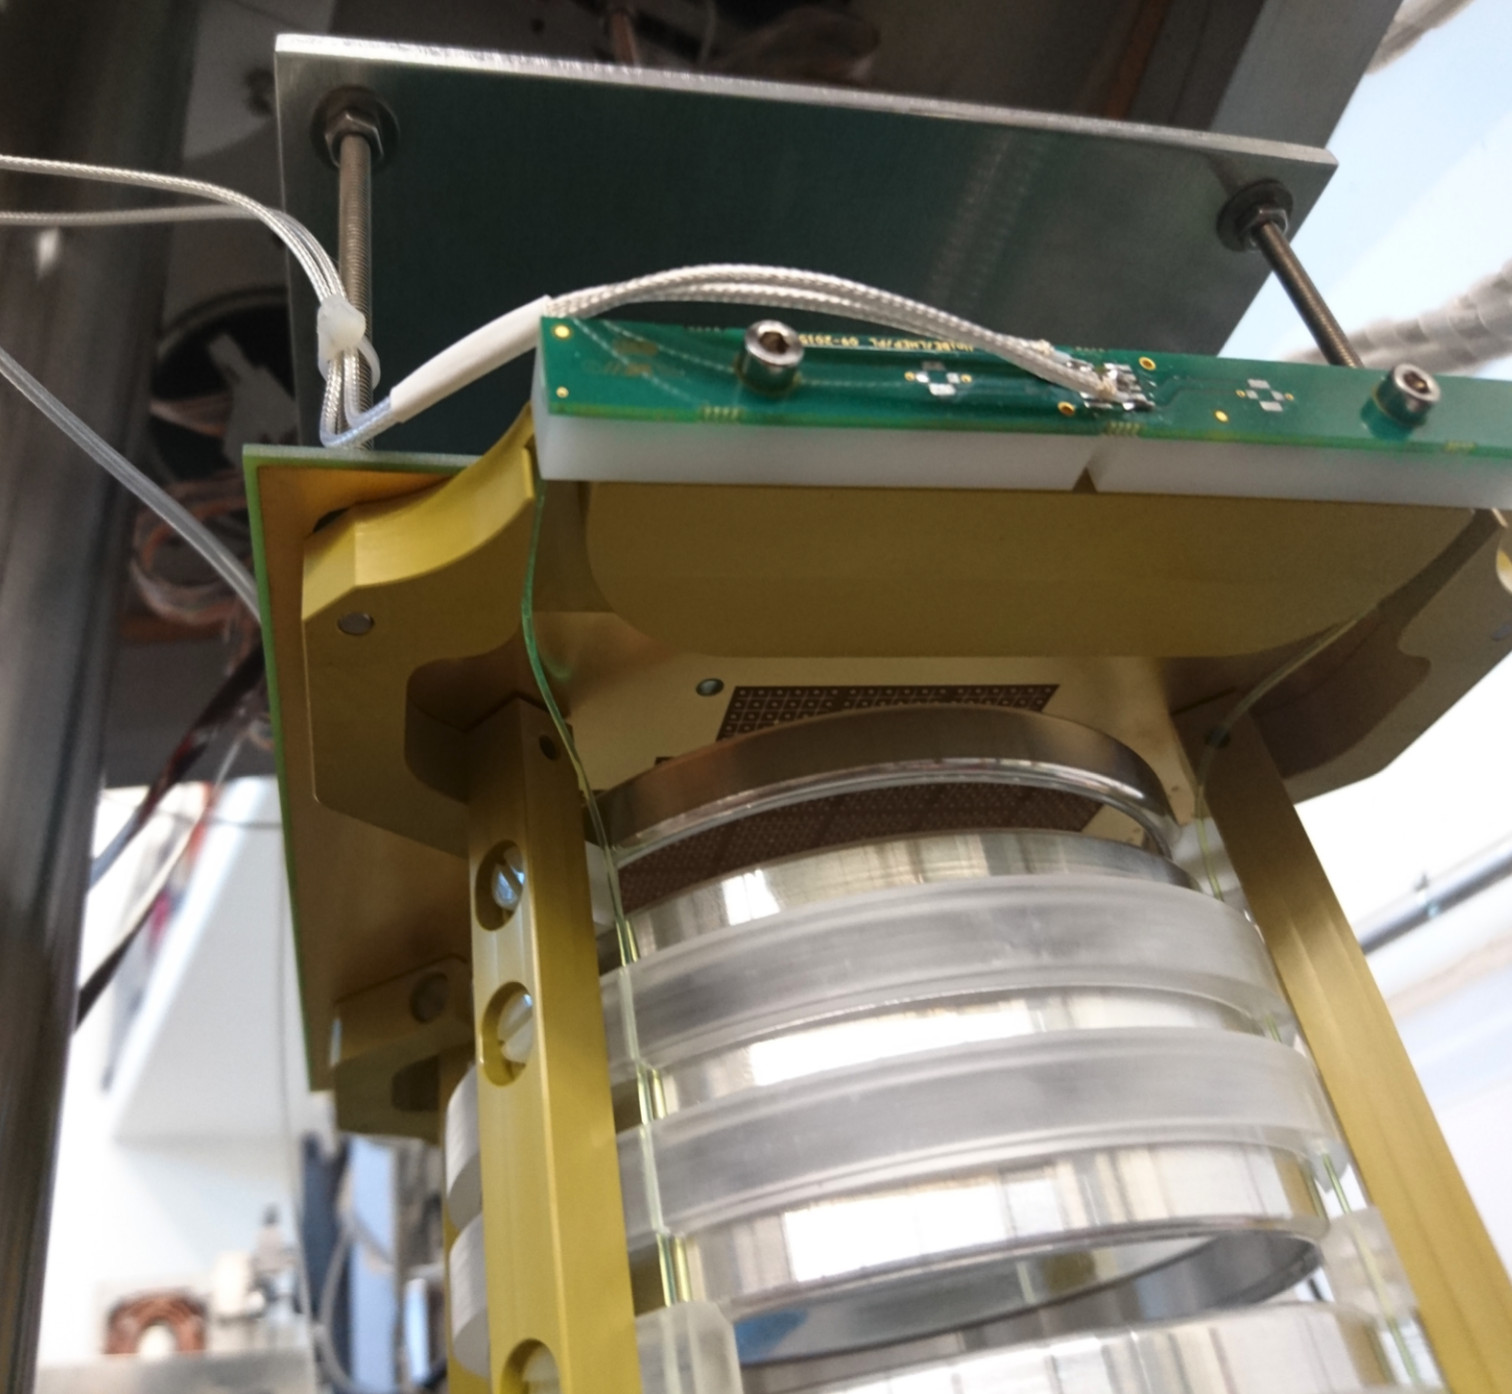
\includegraphics[width=0.62\linewidth]{viper/viper_sipm}
	\caption{\small  Left: Photograph of the  pixel demonstration \gls{tpc} at \gls{help}, with the \gls{hv} feedthrough.
	Right: Close-up of the light collection system, showing \gls{wls} fibres coupling \glspl{sipm} to the \gls{tpb}-coated light guides.}
	\label{fig:viper_v1per}
\end{figure}

The acrylic rings provide the light collection; their inner surfaces are machine-polished and coated with the \gls{wls} \gls{tpb}. 
The coating method is based on~\cite{TPBcoating}.
\SI{0.5}{\gram} of \gls{tpb} and \SI{0.5}{\gram} of acrylic flakes were dissolved in \SI{50}{\milli\liter} of toluene and then mixed with \SI{12}{\milli\liter} of ethanol, which serves to increase the coating homogeneity. 
Three layers of the coating were applied by hand, with a fine brush. 

\SI{1}{\milli\metre} diameter \gls{wls} fibres (Kuraray Y11(200)M) couple the acrylic rings to the four Hamamatsu S12825-050P \glspl{sipm} mounted close to the anode, see Figure~\ref{fig:viper_v1per}. 
The \glspl{sipm} and their front-end electronics were adapted from those developed at \gls{help} for the \glspl{crt} used in \uboone{} and \sbnd{}~\cite{crt, crt_feb}.
For operation in \lar{}, the \gls{sipm} bias voltages had to be reduce from $\approx$~\SI{70}{\volt} to \SI{53}{\volt}, in order to limit the gain.   
In the front-end electronics, two coincidences of two out of the four \glspl{sipm} are formed and combined by means of a logic \textit{OR} operation. 
This coincidence is used in order to improve trigger purity.


\subsection{Ancillary Infrastructure}
\label{sec:ac_viper_infrastructure}

The pixel demonstration \gls{tpc} is housed in a double-bath vacuum-insulated cryostat with the outer bath open to atmosphere.
A diameter of \SI{50}{\centi\metre} and a height of \SI{110}{\centi\metre} give an inner volume of $\approx \SI{200}{\litre}$ of \lar{}.
This is the same cryostat that was used for the \gls{hv} studies described in Section~\ref{sec:studies_hv}.
The \lar{} filtering method is the same as described in~\cite{2photonAbs}, with \lar{} filtered first on filling through a pair of Oxysorb-Hydrosorb filters, and then recirculated through a single custom-made filter containing both activated copper and silica gel.
\lar{} purity is estimated to be in accordance with~\cite{2photonAbs}, with impurity concentrations $\sim{\SI{1}{ppb}}$ of oxygen-equivalent, which corresponds to a charge lifetime of \SI{290+-30}{\micro\second}.

The \gls{hv} feedthrough remains unchanged from the breakdown studies (Section~\ref{sec:studies_hv}); a PET-C polymer dielectric capable of potentials as high as \SI{-130}{\kilo\volt}.
A low-pass filter was added between the power supply and feedthrough, which consists of an \SI{800}{\pico\farad} decoupling capacitor grounded between two \SI{100}{\mega\ohm} resistors connected in series, i.e.\ an RC low-pass filter with an additional protection resistor at the output.
For proper insulation, the whole assembly is submerged in transformer oil.


\subsection{\glsentrylong{snr}}
\label{sec:ac_viper_snr}
\glsreset{snr}

To assess the \gls{snr}, dedicated noise data was taken employing a \SI{5}{\hertz} random trigger.
The data of \num{5000} events was combined.
Subsequently, all pixel and \gls{roi} channels were combined separately and filled into respective amplitude distribution histograms.
Finally, the standard deviation of the noise was calculated by fitting a Gaussian to the amplitude distribution.
This value was used to calculate the noise for pixel and \gls{roi} channels according to
\begin{IEEEeqnarray}{rCl}
	\m{SNR} & = & \frac{S}{\sigma} \qc
	\label{eq:viper_snr}
\end{IEEEeqnarray}
where $S$ is the signal and $\sigma$ is the noise standard deviation from the Gaussian fit.
As can be seen in the left plot in Figure~\ref{fig:viper_unfilteredRawData}, one of the pixel channels is significantly noisier in comparison to others, likely caused by a broken preamplifier.
Therefore, this channel was blinded for the \gls{snr} calculations.
The resulting equivalent noise charge is \SI{1095}{\elementarycharge} for the pixel channels and \SI{982}{\elementarycharge} for the inductive \gls{roi} channels

The signal $S$ is often taken for a \gls{mip} as this is at the lower end of the signal range interesting for neutrino physics.
Getting a clean \gls{mip} sample from experimental data requires a calibrated reconstruction which was not available at the time of writing.
Therefore, the \gls{mip} signal was estimated from theory assuming an energy loss of \SI{2.1}{\mega\electronvolt\per\centi\metre} (see Section~\ref{sec:nu-detection_fs}).
This can be converted to charge loss using the energy required to produce one electron-ion pair from Table~\ref{tab:lartpc_larprop}: $W_{\m{i}} = \SI{23.6}{\electronvolt\per\elementarycharge}$.
Additionally, charge recombination, diffusion and lifetime need to be taken into account (see Section~\ref{sec:lartpc_lar}).
The recombination factor was measured by \icarus{}~\cite{icarusReco} and \argoneut{}~\cite{argoneutReco} and found to be $R_{\m{c}} \approx 0.7$ for a drift field of $\SI{1}{\kilo\volt\per\centi\meter}$.
With \AT{}~\cite{AT}, \gls{help} measured a transverse diffusion coefficient $D_{\m{T}} = \SI{5.3}{\centi\metre\squared\per\second}$ at \SI{0.25}{\kilo\volt\per\centi\metre} while Gushchin et al.~\cite{gushchin} report a value of $D_{\m{T}} = \SI{13}{\centi\metre\squared\per\second}$ at \SI{1}{\kilo\volt\per\centi\metre}.
Even using the more conservative value, this results in a transverse spread of $\approx \SI{0.9}{\milli\metre}$ for the pixel demonstrator drift time of $t = \SI{281}{\micro\second}$, according to Equation~\eqref{eq:lartpc_lar-diff}.
This value lies well below the pixel pitch of $d_{\m{p}} = \SI{2.54}{\milli\metre}$.
Considering that the longitudinal component is smaller than the transverse ~\cite{lngDet}, diffusion is neglected completely for these calculations.
Finally, the lifetime of \SI{290}{\micro\second} will result in the reduction of charge by a factor of $\approx\num{0.38}$ over the full drift distance (Equation~\eqref{eq:lartpc_lar-lifetime}).
Combining this, the signal is 
\begin{IEEEeqnarray}{rCl}
	S & = & \dv{E}{x}_{\m{MIP}} \frac{R_{\m{c}} d_{\m{p}}}{W_{\m{i}}} = \SI{15821}{\elementarycharge} \qc
\end{IEEEeqnarray}
for a charge deposited adjacent to the readout plane, and $S = \SI{6004}{\elementarycharge}$ for a charge deposited adjacent to the cathode.

Table~\ref{tab:viper_snr} lists the \gls{snr} values obtained from these signal values and the aforementioned measured equivalent noise charge, using Equation~\eqref{eq:viper_snr}.

\begin{table}[htb]
	\centering
	\caption{\gls{snr} values obtained from Equation~\eqref{eq:viper_snr} using the theoretical signal of a \gls{mip} at the readout plane or cathode, respectively combined with the average equivalent noise charge for pixel and \gls{roi} channels obtained from measurements.}
	\label{tab:viper_snr}
	\begin{tabu} to \textwidth {llS}
		\toprule
		Channel &	\gls{mip} at &		{\gls{snr}} \\
		\midrule
		Pixel &		Readout plane &	14 \\
		Pixel &		Cathode &		5.5 \\
		\gls{roi} &		Readout plane &	16 \\
		\gls{roi} &		Cathode &		6.1 \\
		\bottomrule
	\end{tabu}
\end{table}


\subsection{3D track reconstruction}
\label{sec:ac_viper_3d}

To demonstrate 3D track reconstruction, several thousand cosmic ray events were collected, many of which are \glspl{mip}, mostly muons.
The charge readout was triggered by the light readout described above.

The reconstruction procedure comprises five steps: noise filtering, hit finding, hit matching, ambiguity rejection, and track fitting.
These steps are explained in the following and depicted in Figures~\ref{fig:viper_unfilteredRawData} through~\ref{fig:viper_kalman}, all taken from the same \gls{mip} (cosmic muon) event.

In the first step, a noise-filtering algorithm is applied to the raw data.
As can be seen from Figure~\ref{fig:viper_unfilteredRawData}, the noise is largely correlated across all the channels.
\footnote{Due to the much higher signal levels, the noise is barely visible on the pixel channels on the left.}
This common-mode correlation can be exploited by the noise filter algorithm.
The following is done separately for the all pixel and \gls{roi} channels of each event.
Similarly to the \gls{snr} calculation, all samples are filled into an amplitude distribution histogram for each channel, and subsequently fitted with a Gaussian.
A noise band is defined per channel with its centre equal to the mean of the Gaussian and its width equal to the standard deviation multiplied by a tunable scaling factor.
The amplitudes of all channels within the corresponding noise band are then averaged for each sample.
Finally, this average is subtracted from each channel at the corresponding sample.
This technique was chosen because it effectively suppresses the dominating common mode noise.
At the same time, spurious signals produced by high amplitudes from collected charge distorting the average are kept to a minimum by only accepting values within the noise band.
The effectiveness of the filtering can be seen in Figure~\ref{fig:viper_filteredRawData}, which shows the same data as Figure~\ref{fig:viper_unfilteredRawData} post filtering.

\begin{figure}[htb]
	\centering
	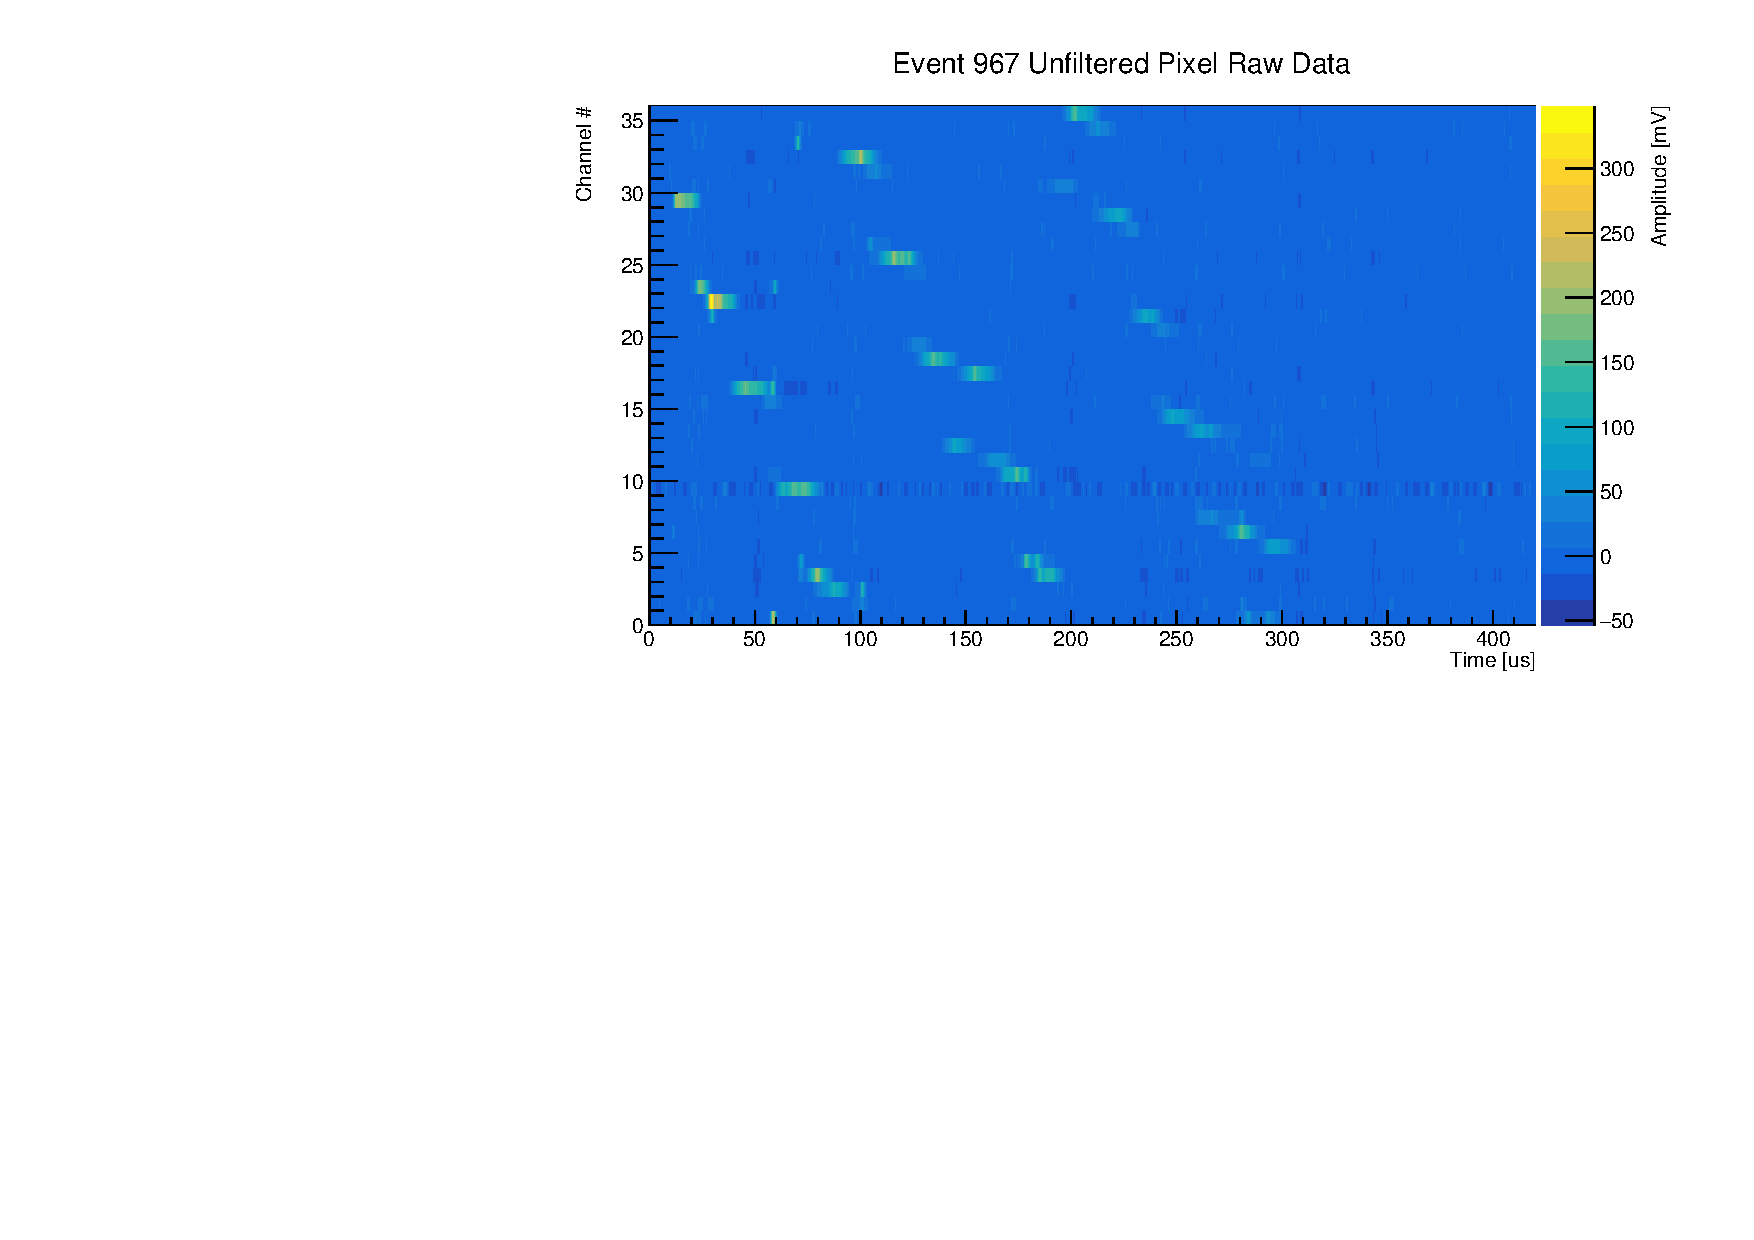
\includegraphics[width=\textwidth]{viper/event967_rawUnfilteredPixel}\\
	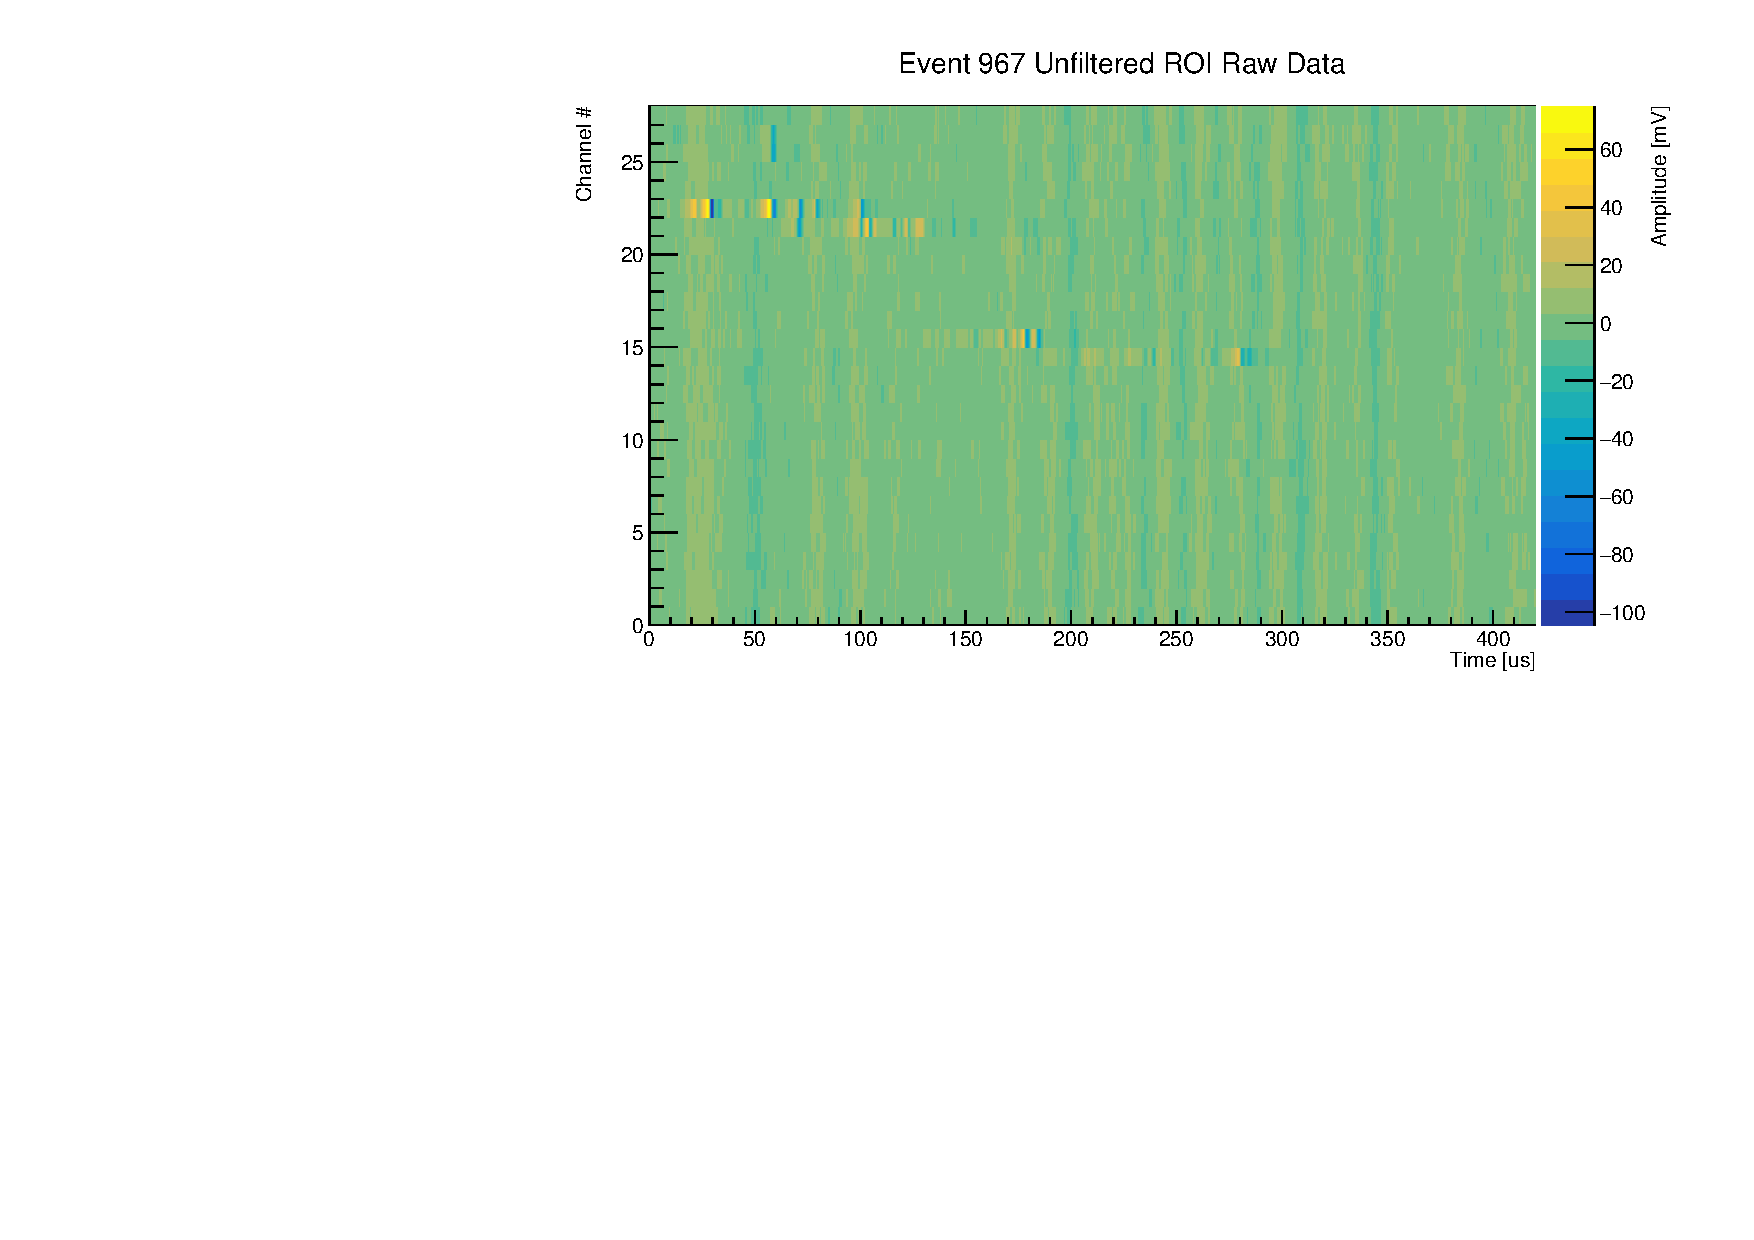
\includegraphics[width=\textwidth]{viper/event967_rawUnfilteredROI}
	\caption{Unfiltered raw data of a typical \gls{mip} event (the same event as in Figures~\ref{fig:viper_unfilteredRawData}~through~\ref{fig:viper_kalman}). The top plot shows pixel data while the bottom plot shows \gls{roi} data.}
	\label{fig:viper_unfilteredRawData}
\end{figure}

\begin{figure}[htb]
	\centering
	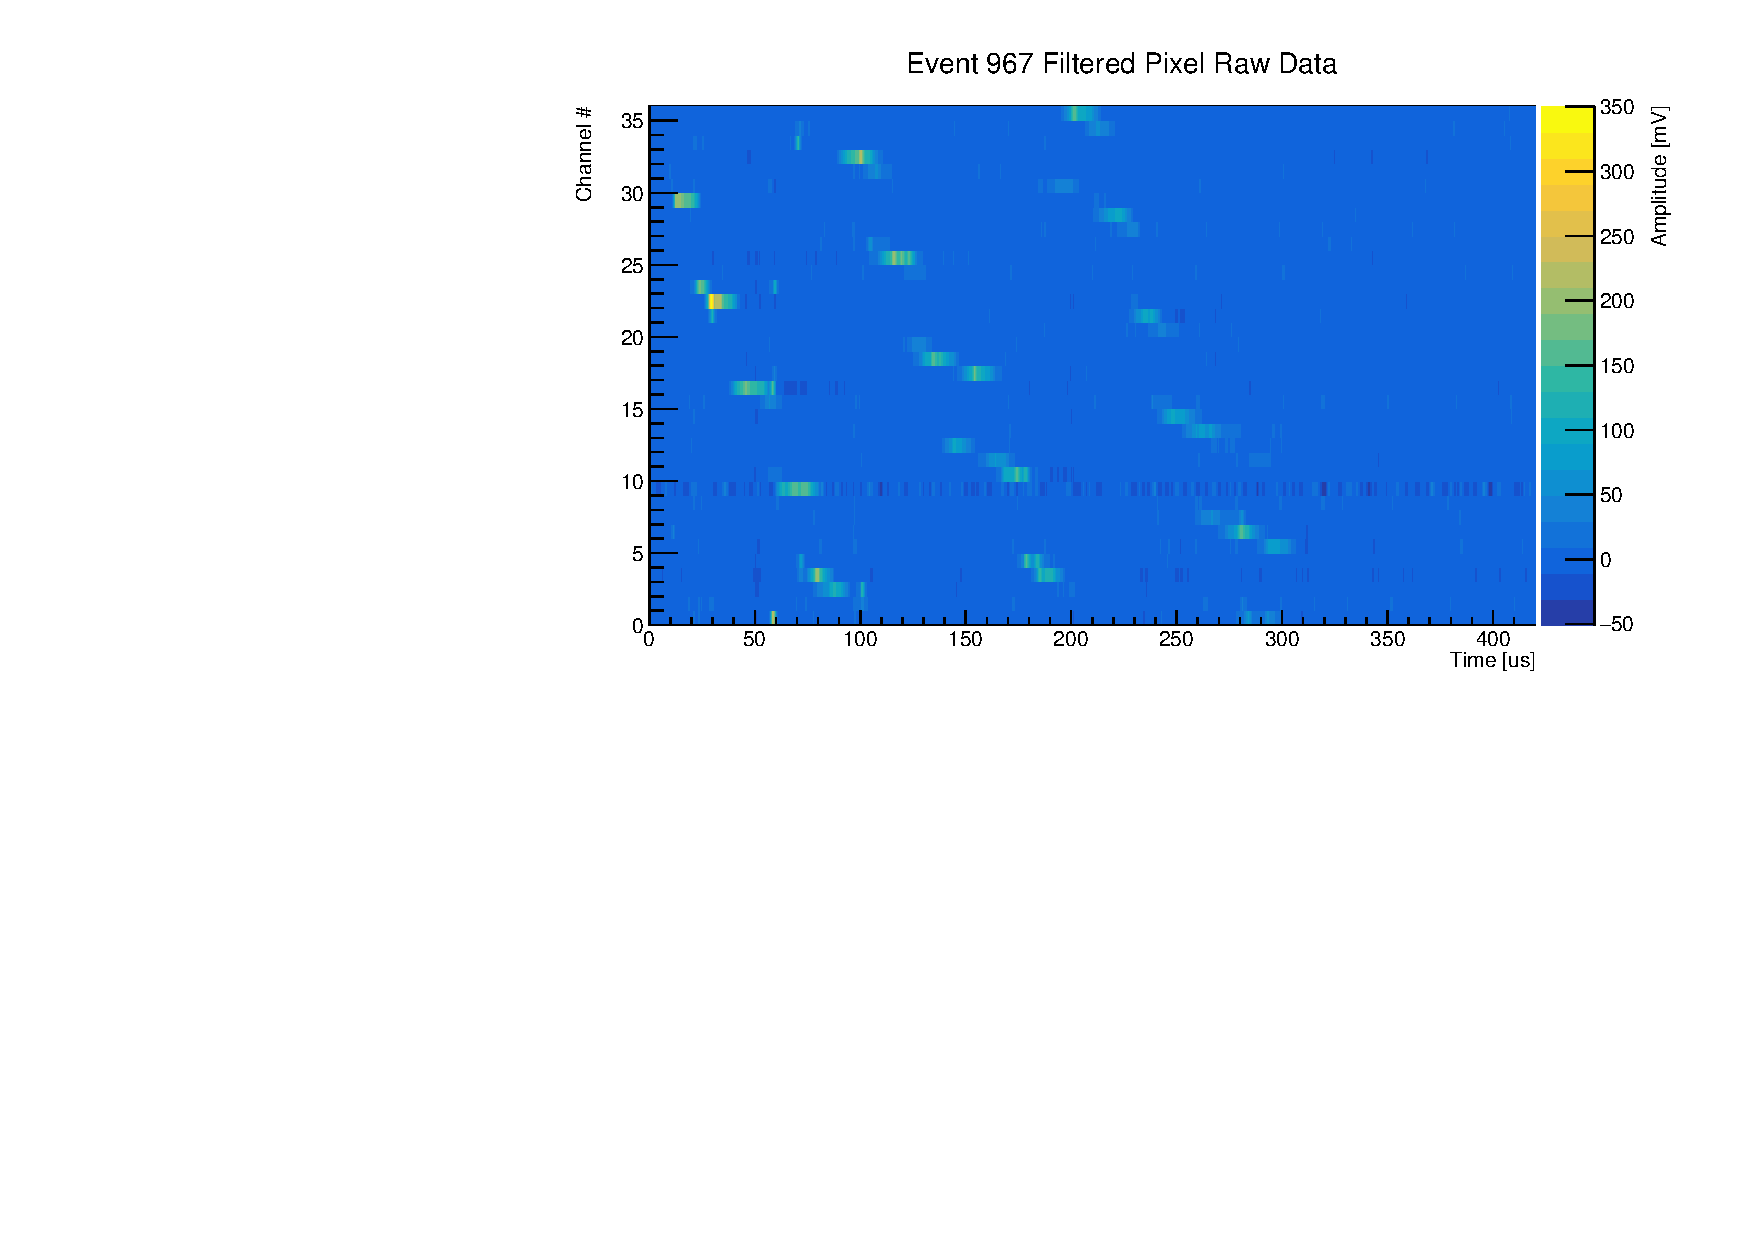
\includegraphics[width=\textwidth]{viper/event967_rawFilteredPixel}\\
	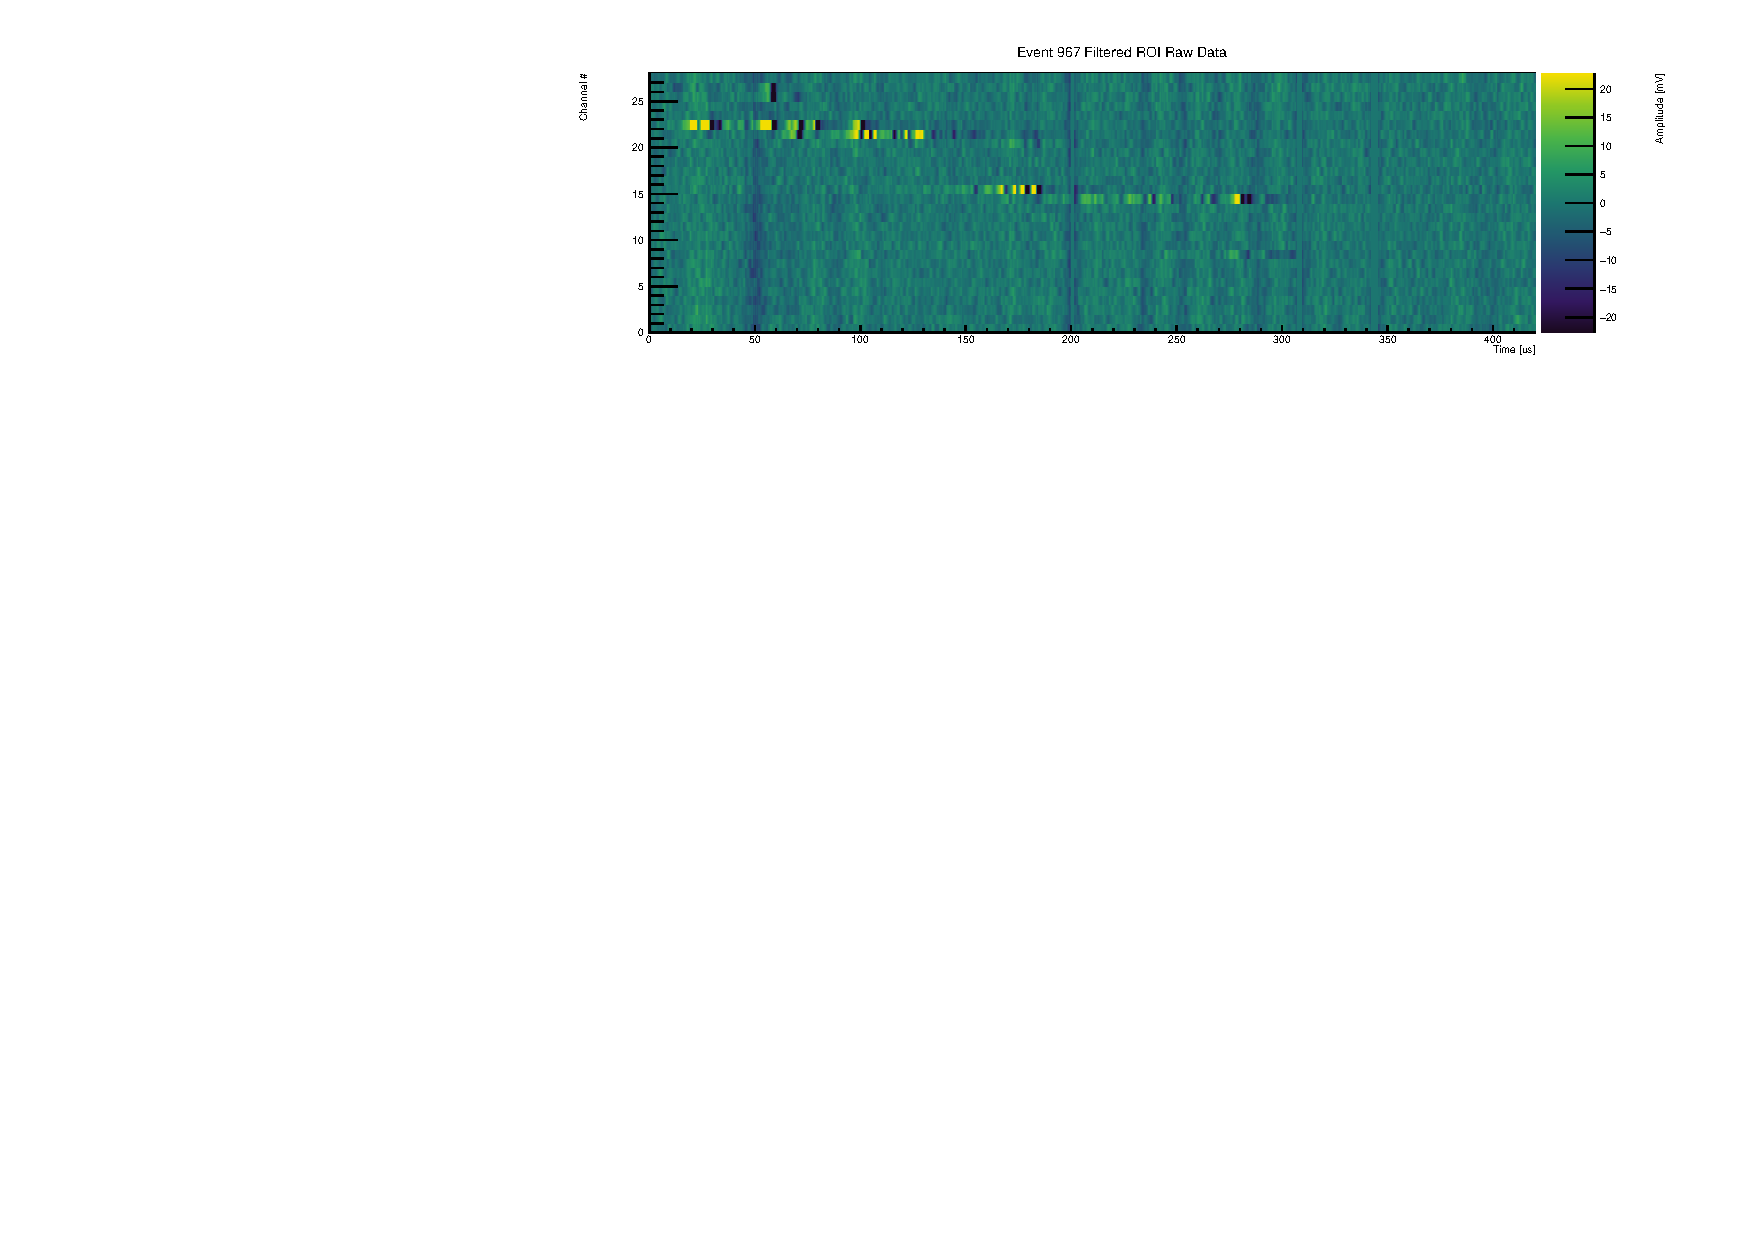
\includegraphics[width=\textwidth]{viper/event967_rawFilteredROI}
	\caption{Filtered data of a typical \gls{mip} event (the same event as in Figures~\ref{fig:viper_unfilteredRawData}~through~\ref{fig:viper_kalman}).
	The top plot shows pixel data while the bottom plot shows \gls{roi} data}
	\label{fig:viper_filteredRawData}
\end{figure}

The second step applies a recursive pulse finding algorithm.
The following is performed for each channel independently.
Most thresholds employed by the pulse finder are, again, defined in terms of noise amplitude.
Therefore, noise mean and standard deviation are recalculated after noise filtering.
A peak threshold is defined by multiplying the noise standard deviation by a variable scaling factor and adding the noise mean.
Then, the sample with the highest amplitude is found.
If it is below threshold, the process stops and proceeds to the next channel.
Otherwise, the pulse is scanned in positive and negative directions until it crosses respective lower noise thresholds.
After this, the whole pulse is deleted from the data and the process starts over with finding the new maximum sample and checking it against the peak threshold.
For stability reasons, the peak threshold relative to noise levels is compared against an absolute threshold and the higher of the two is applied.
The search is extended to the negative pulse for the bipolar \gls{roi} pulses.
The different thresholds employed and samples found by this process are illustrated in Figure~\ref{fig:viper_hitFinder}.

\begin{figure}[htb]
	\centering
	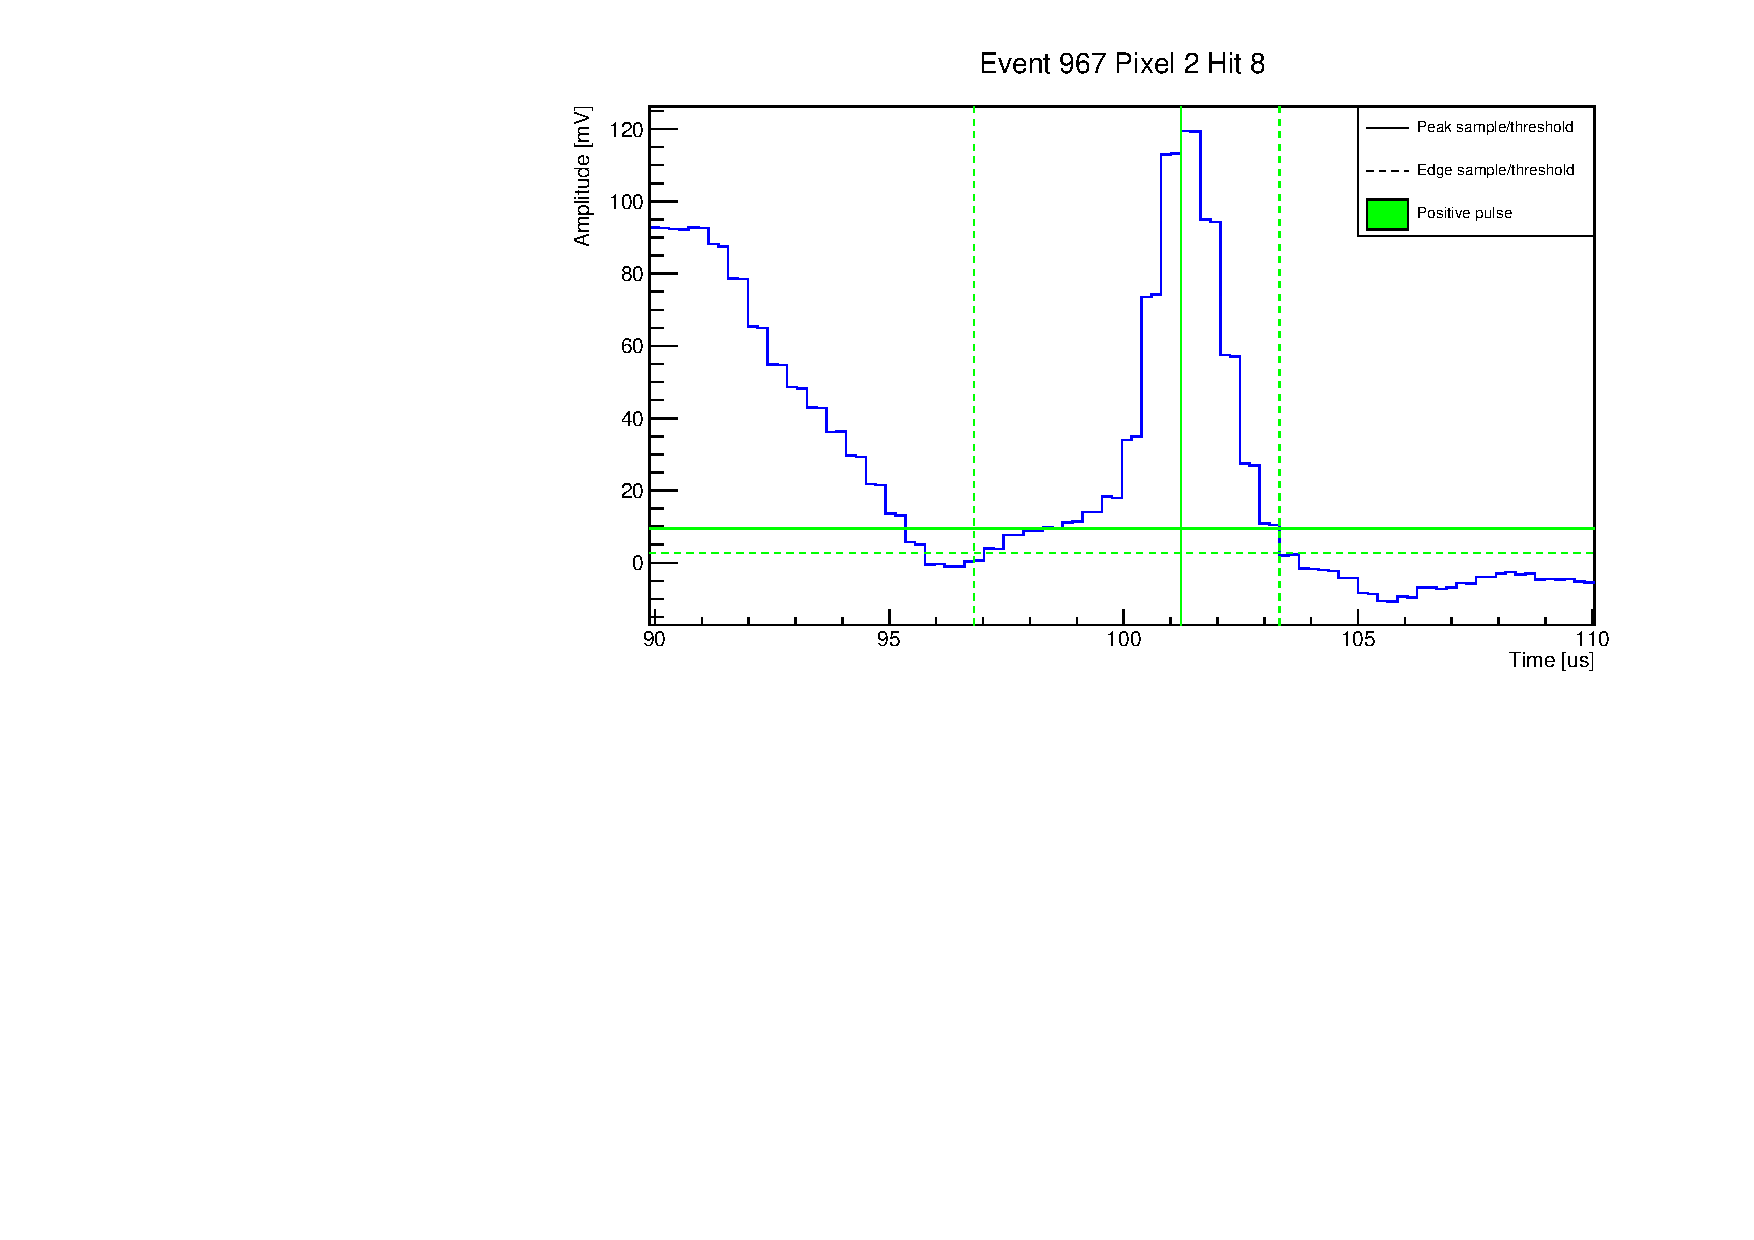
\includegraphics[width=\textwidth, page=1]{viper/event967_pixel2_hit8}\\
	\includegraphics[width=\textwidth, page=3]{viper/event967_pixel2_hit8}
	\caption{Pulse shapes of a single pixel (top) and \gls{roi} (bottom) hit of a typical \gls{mip} event (the same event as in Figures~\ref{fig:viper_unfilteredRawData}~through~\ref{fig:viper_kalman}).
	Superimposed are the thresholds of the hit finder algorithm. Horizontal lines represent thresholds: the solid is the minimum threshold required to be crossed for a pulse to be detected, and dashed are the thresholds used to detect the pulse edges.
	Vertical lines represent the corresponding detected peak/edge samples.
	Colour indicates a positive (green) or negative (red) pulse, or a zero crossing (yellow).}
	\label{fig:viper_hitFinder}
\end{figure}

Identified pulses are then combined into 3D hits by matching pixels pulses to \gls{roi} pulses.
For this proof of concept, this is done rather primitively by matching any pulses coinciding in time.
In Figure~\ref{fig:viper_hitFinder}, a pixel and \gls{roi} pulse are matched if their time slices, defined by the vertical dashed lines, overlap.
This third step results in a rather high amount of ambiguities but assures that no hits are missed.

To resolve the ambiguities, a Principal Component Analysis (PCA) is applied to the 3D space points in a fourth step.
This technique is well established and described in literature, e.g.~\cite{pca}.
Therefore, it shall be explained here only briefly.
The basic idea is to calculate three orthogonal eigenvectors of the 3D space point cloud.
A graphic interpretation of these eigenvectors are the three axis of an ellipsoid fitted to the data points.
In case the points form a track, one of these eigenvectors will have a much higher eigenvalue than the other two.
This eigenvector is taken as an estimate for the track direction.
The ambiguities can be resolved by selecting the one closest to the track estimate.
Furthermore, this procedure can be used to recursively reject outliers by forming a cylinder around the track estimate with a radius proportional to the second largest eigenvalue.
All hits outside this cylinder are rejected.
The procedure can be repeated by rerunning the PCA on the remaining points and performing another outlier rejection.
In a later stage of reconstructing more complex events, this algorithm can potentially be used to cluster 3D space points in order to separate multiple tracks.
The PCA ambiguity rejection is illustrated in Figure~\ref{fig:viper_pca}.

\begin{figure}[htb]
	\centering
	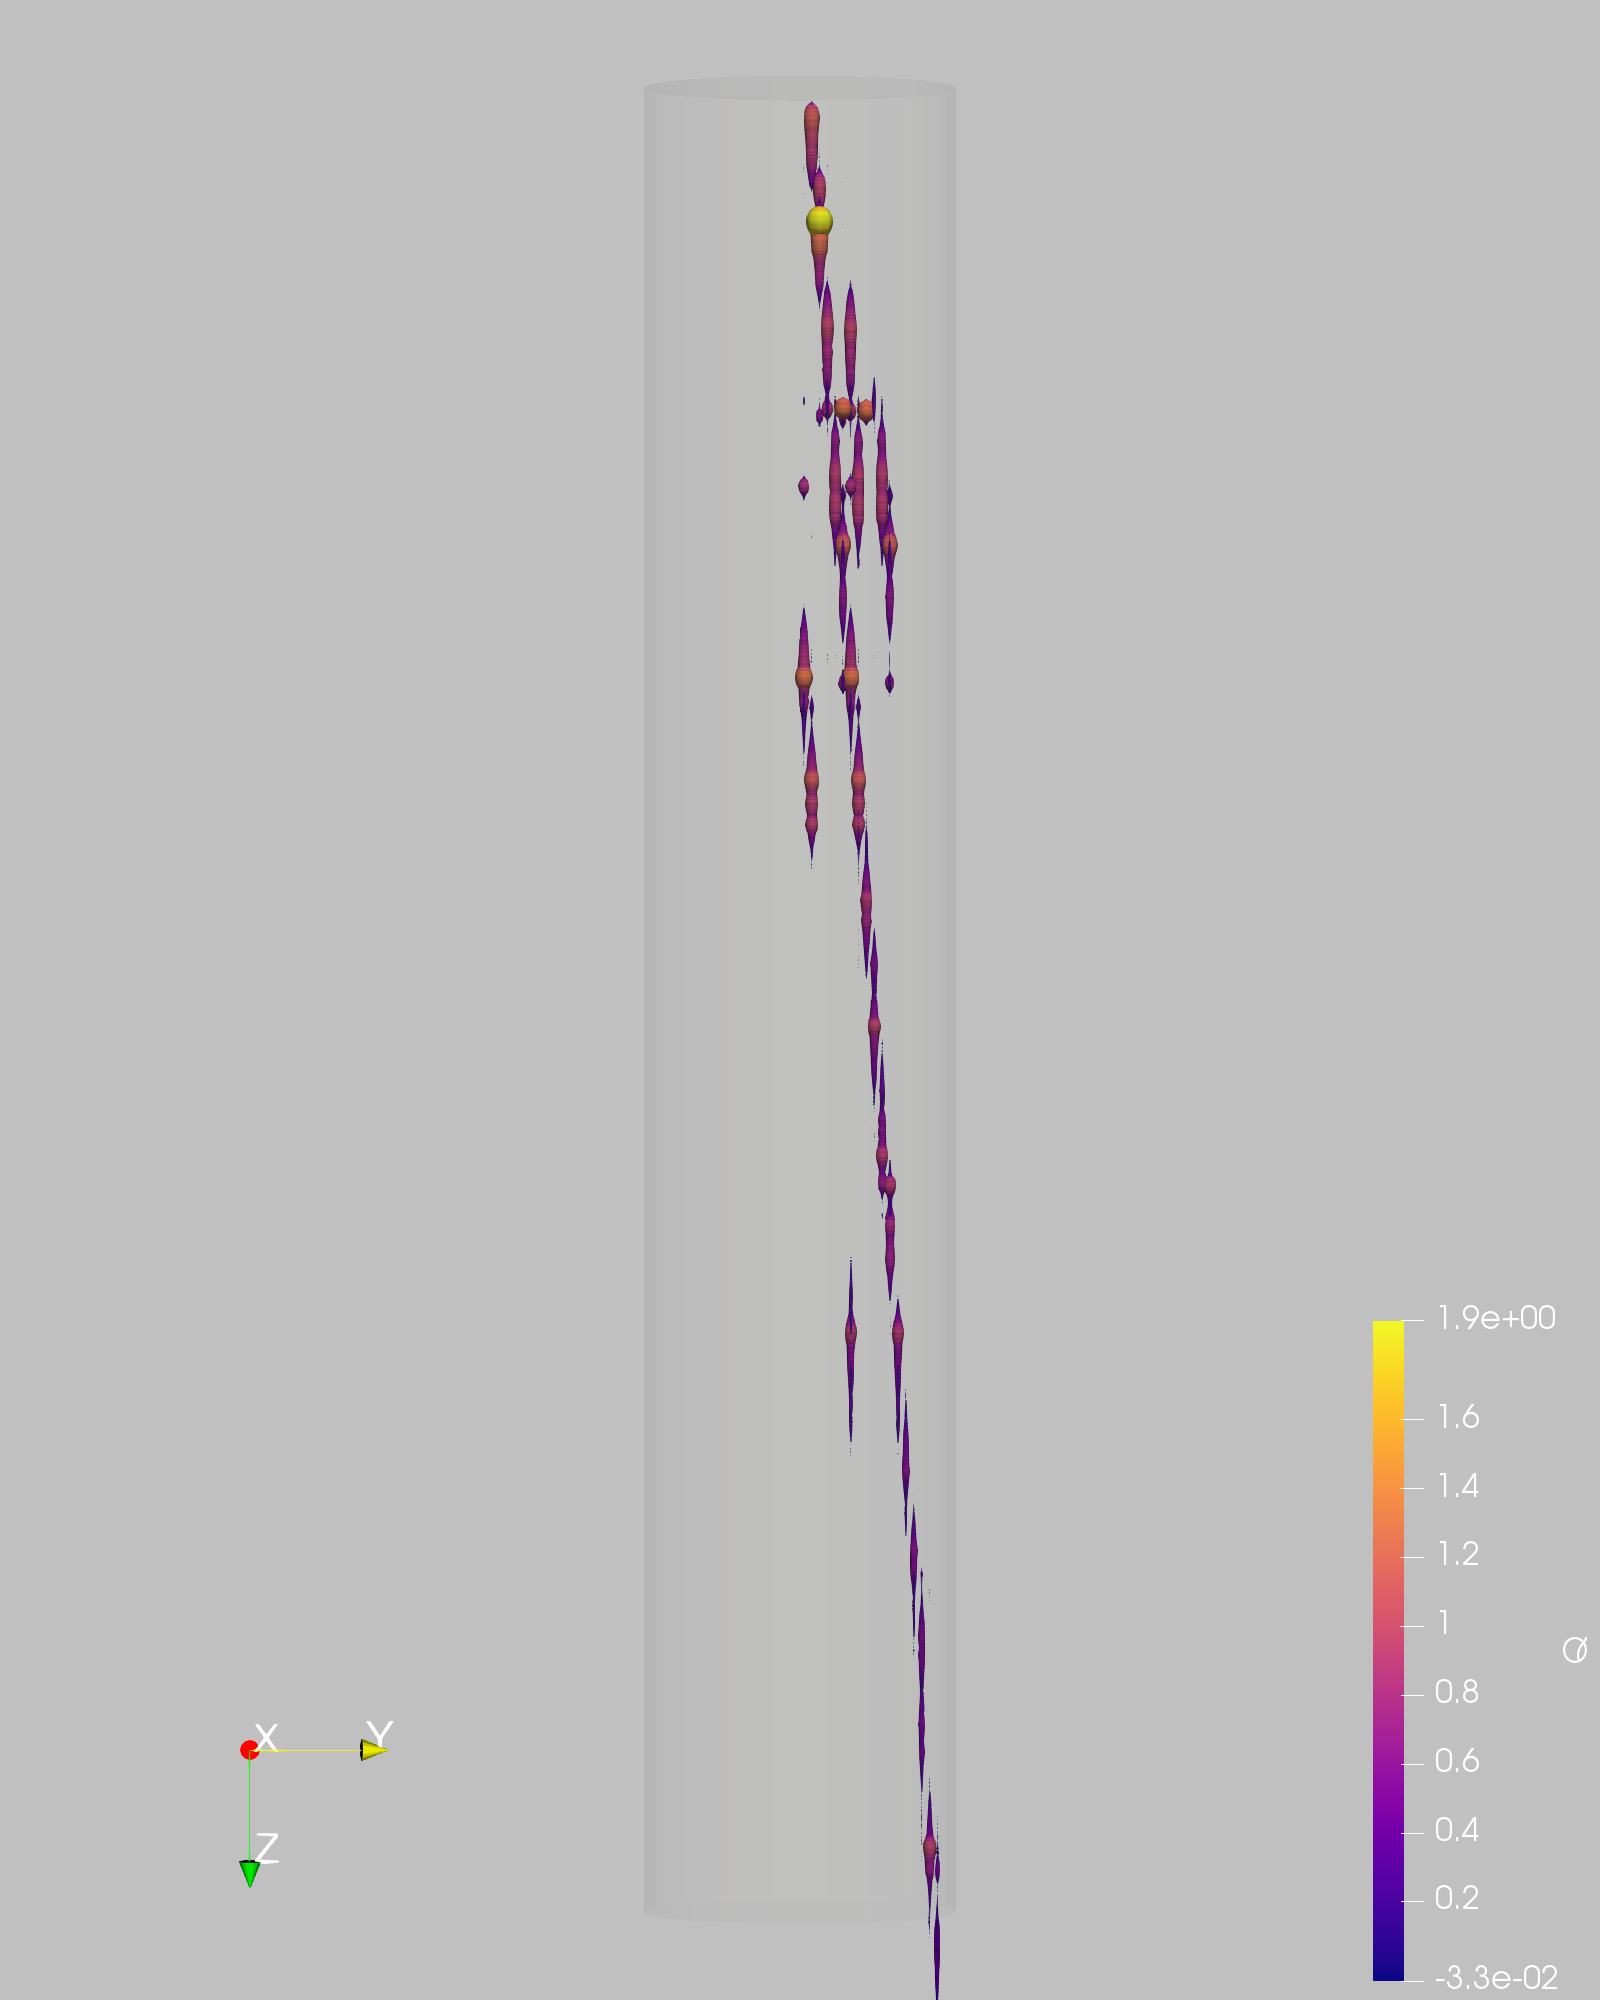
\includegraphics[viewport=600 0 1000 2000, clip, height=\textwidth, angle=90]{viper/event967_pulses_q} \\
	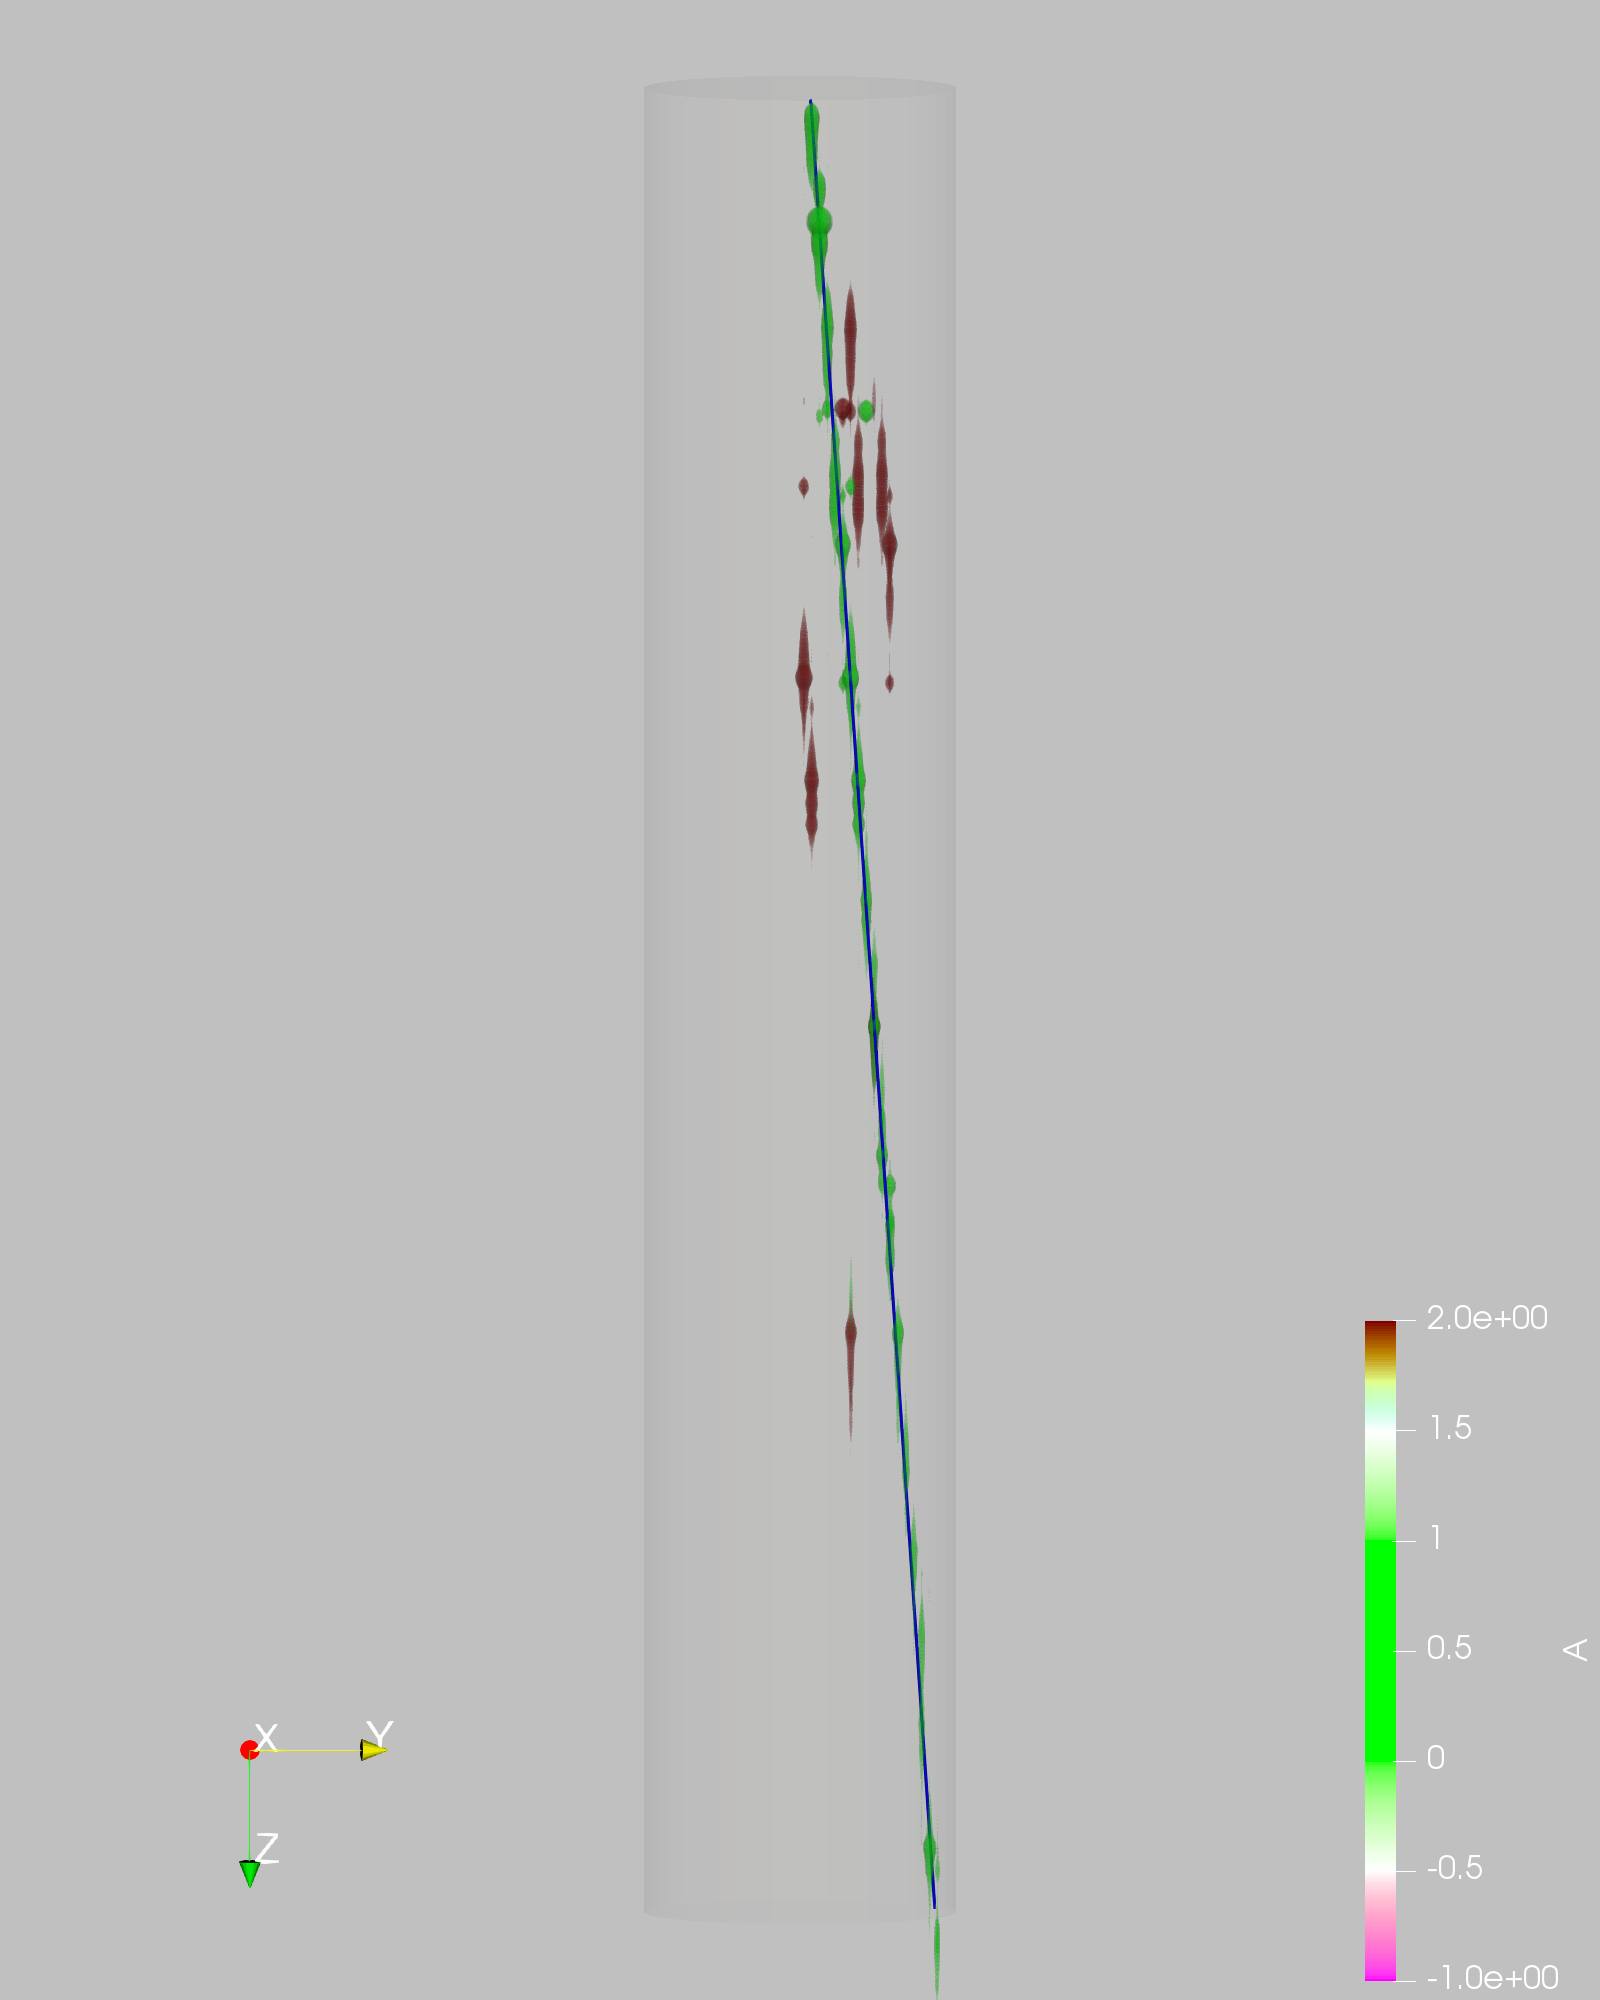
\includegraphics[viewport=600 0 1000 2000, clip, height=\textwidth, angle=90]{viper/event967_pulses_a_pca} \\
	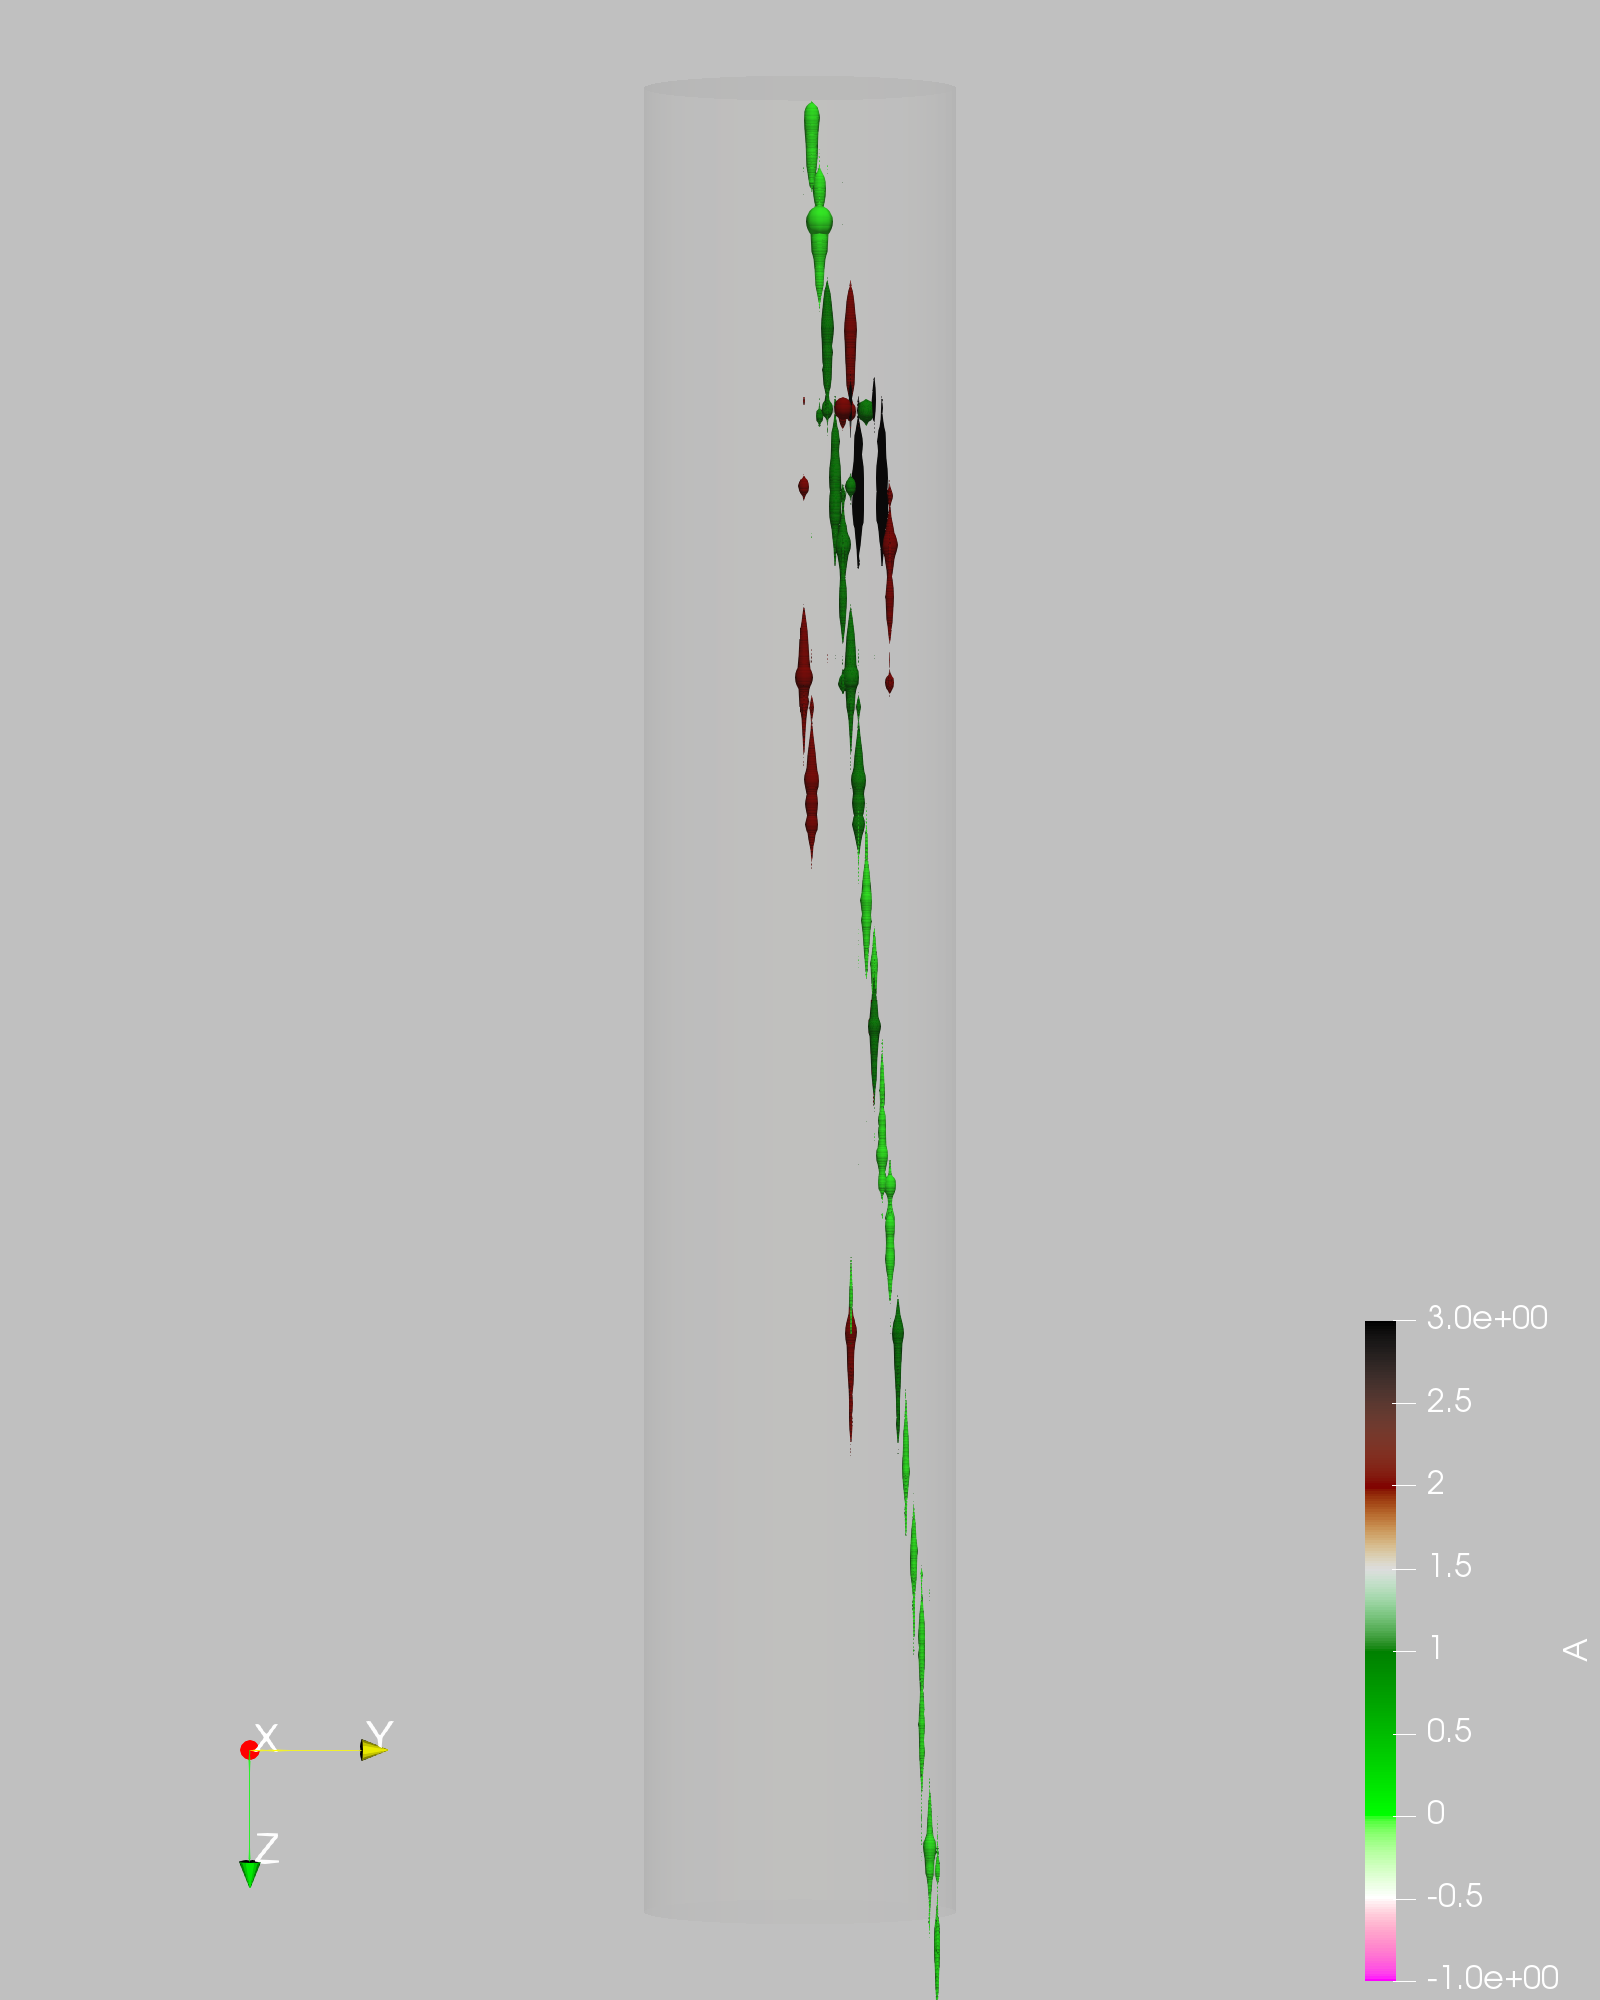
\includegraphics[viewport=600 0 1000 2000, clip, height=\textwidth, angle=90]{viper/event967_pulses_a_det}
	\caption{Reconstructed 3D hits from the hit finder.
		The passing particle is most likely a cosmic \Pgm entering from the left (the same event as in Figures~\ref{fig:viper_unfilteredRawData}~through~\ref{fig:viper_kalman}).
		Drift direction is from right to left.
		Pulse shape is encoded as thickness.
		In the top plot, colour codes the amount of collected charge.
		The middle plot illustrates the ambiguity resolution employing a principal component analysis.
		Green hits are accepted while dark red ones are rejected.
		This is achieved by selecting the ambiguity closest to the eigenvector of the point cloud with the largest eigenvalue, represented by the blue line.
		In the bottom plot, the degree of ambiguity is colour-coded: Light green are unambiguous hits while dark green are selected solutions of ambiguous hits.
		Dark red through black are rejected solutions of ambiguous hits where darker colour represents a higher degree of ambiguity.
		As this is a quite clean track with only few short $\delta$ rays, there are no outliers rejected other than the multiplexing ambiguities.}
	\label{fig:viper_pca}
\end{figure}

The final step consists of a Kalman filter.
For this, the well-established \gls{genfit} package~\cite{genfit1, genfit2} was used.
Ionisation losses and multiple scattering are taken into account.
The particle is assumed to be a minimum-ionising muon with an initial momentum of \SI{260}{\mega\electronvolt\per\clight} in the direction of the track estimate from the PCA.
A recursive algorithm capable of dealing with outliers was chosen, a so-called \emph{deterministic annealing filter}.
This works by assigning successively lower weights to outliers with each recursion step.
For more details, see the respective publications~\cite{genfit1, genfit2}.
The resulting track is shown in Figure~\ref{fig:viper_kalman}.

\begin{figure}[htb]
	\centering
	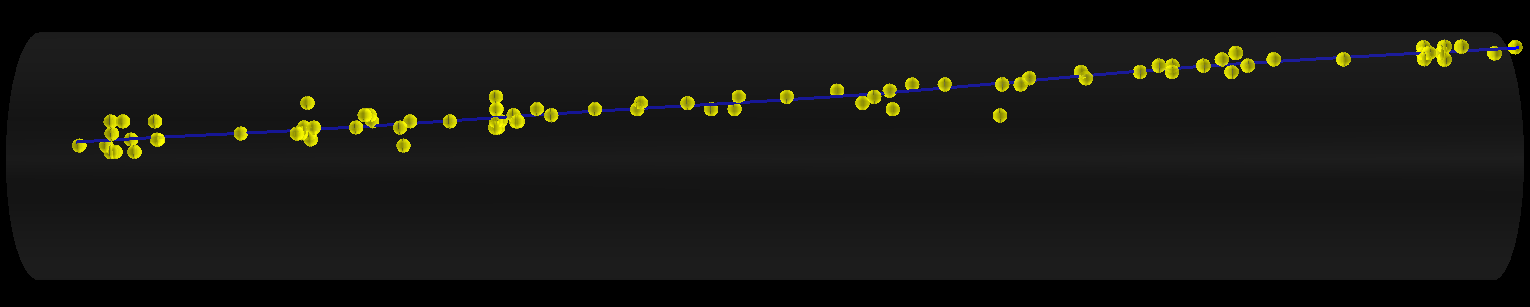
\includegraphics[width=\textwidth]{viper/event967_kalman}
	\caption{Track fitted by the Kalman filter.
	The \gls{tpc} volume is shown in faint grey.
	The passing particle is most likely a cosmic \Pgm entering from the left (the same event as in Figures~\ref{fig:viper_unfilteredRawData}~through~\ref{fig:viper_kalman}).
	Drift direction is from right to left.
	The yellow points are the input to the Kalman filter, the accepted hits from the principal components analysis.
	Blue is the output, a fitted track taking into account ionisation losses and multiple scattering in \lar{}.}
	\label{fig:viper_kalman}
\end{figure}

Technically, the Kalman filter would be capable of fitting the particle momentum or even particle type to the data.
At the time of this writing, this is not implemented yet.
In particular, the momentum stays roughly at the initial guess of \SI{260}{\mega\electronvolt\per\clight}, assuming a minimum ionising muon in \lar{}.
A potential explanation for this is that the resolution of the detector is too low to estimate momentum from multiple scattering.
Another explanation might be the hit finder missing hits due to non-optimal tuning.
Proper tuning of the reconstruction requires a full simulation chain of the detector which is not yet available.
Using data to tune the reconstruction is prone to the introduction of circular biases.
On the other hand, most of the difficulties emerge from the multiplexing ambiguities and their resolution.
While the presented almost full 3D readout has already reduced the reconstruction complexity compared to a classical wire readout, an ambiguity-free readout will make reconstruction another big step easier by completely eliminating the need to resolve ambiguities.


\section{\pixlar{}}
\label{sec:ac_pixlar}

\begin{figure}[htb]
	\centering
	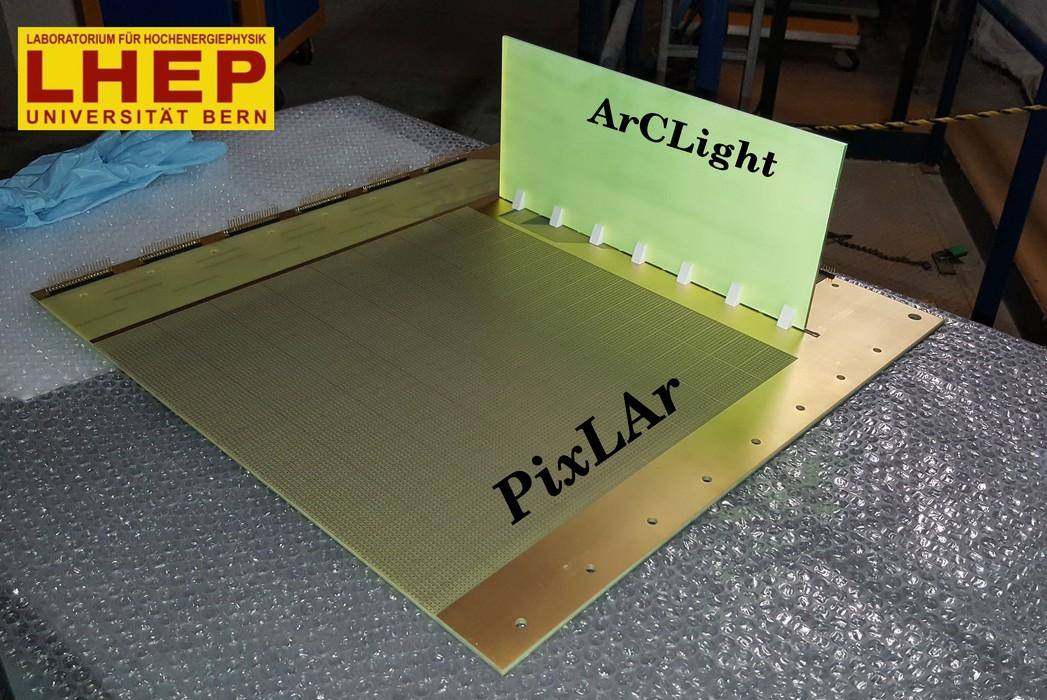
\includegraphics[width=\textwidth]{pixlar/pixlar_arclight}
	\caption{One of the two \pixlar{} readout half planes with the \AL{} module attached.}
	\label{fig:pixlar_arclight}
\end{figure}

After the successful test with cosmic muons at \gls{help}, a bigger prototype of the pixel readout, employing the same multiplexing scheme, was built for a beam exposure in the \lariat{} experiment~\cite{lariat} at \gls{fail}.
\lariat{} consists of the former \argoneut{}~\cite{argoneut} cryostat and \lartpc{} put into a test beam.
The tertiary beam line produces mainly pions and protons as well as electrons, muons and kaons at a lower rate.
Their momentum spectrum can be tuned from \SIrange{0.2}{2.0}{\giga\electronvolt\per\clight}.
\SI{550}{\litre} of \lar{} are contained in a cylindrical cryostat.
It houses a \gls{tpc} with \SI{47}{\centi\metre} drift length and a \SI{40 x 90}{\centi\metre} readout plane parallel to the beam direction, resulting in an active volume of \SI{170}{\litre}.
For the pixel test, called \pixlar{}, the original wire planes were replaced by a \num{120 x 240} pixel readout.
At \SI{3}{\milli\metre} pitch, this gives an instrumented area of \SI{36 x 72}{\centi\metre}.
Due to constraints from the \gls{pcb} manufacturer, the readout plane had to be split into two mirror-symmetric, electrically independent half planes.
Each \num{120 x 120} pixel half plane is divided into \num{8 x 15} \glspl{roi} of \num{15 x 8} pixels each.
The \glspl{roi} are oriented with their longer dimension parallel to the beam direction to reduce the multiplexing ambiguities.
One of the noise mitigation measures implemented for the \gls{help} pixel demonstrator was to use the same differential warm signal path as used by \lariat{}.
Therefore, the charge readout electronics used in \pixlar{} are quite similar to the \AT{} chain described in Section~\ref{sec:studies_electronics_at} after the upgrades.
To trigger on scintillation light, one end of the \gls{tpc} is equipped with a \SI{43 x 15}{\centi\metre} \AL{} module (see Section~\ref{sec:studies_light-col_al}), while the other end features an ARAPUCA~\cite{arapuca} detector for comparison.
Figure~\ref{fig:pixlar_arclight} shows one of the readout half planes with the \AL{} module attached.

\begin{figure}[htb]
	\centering
	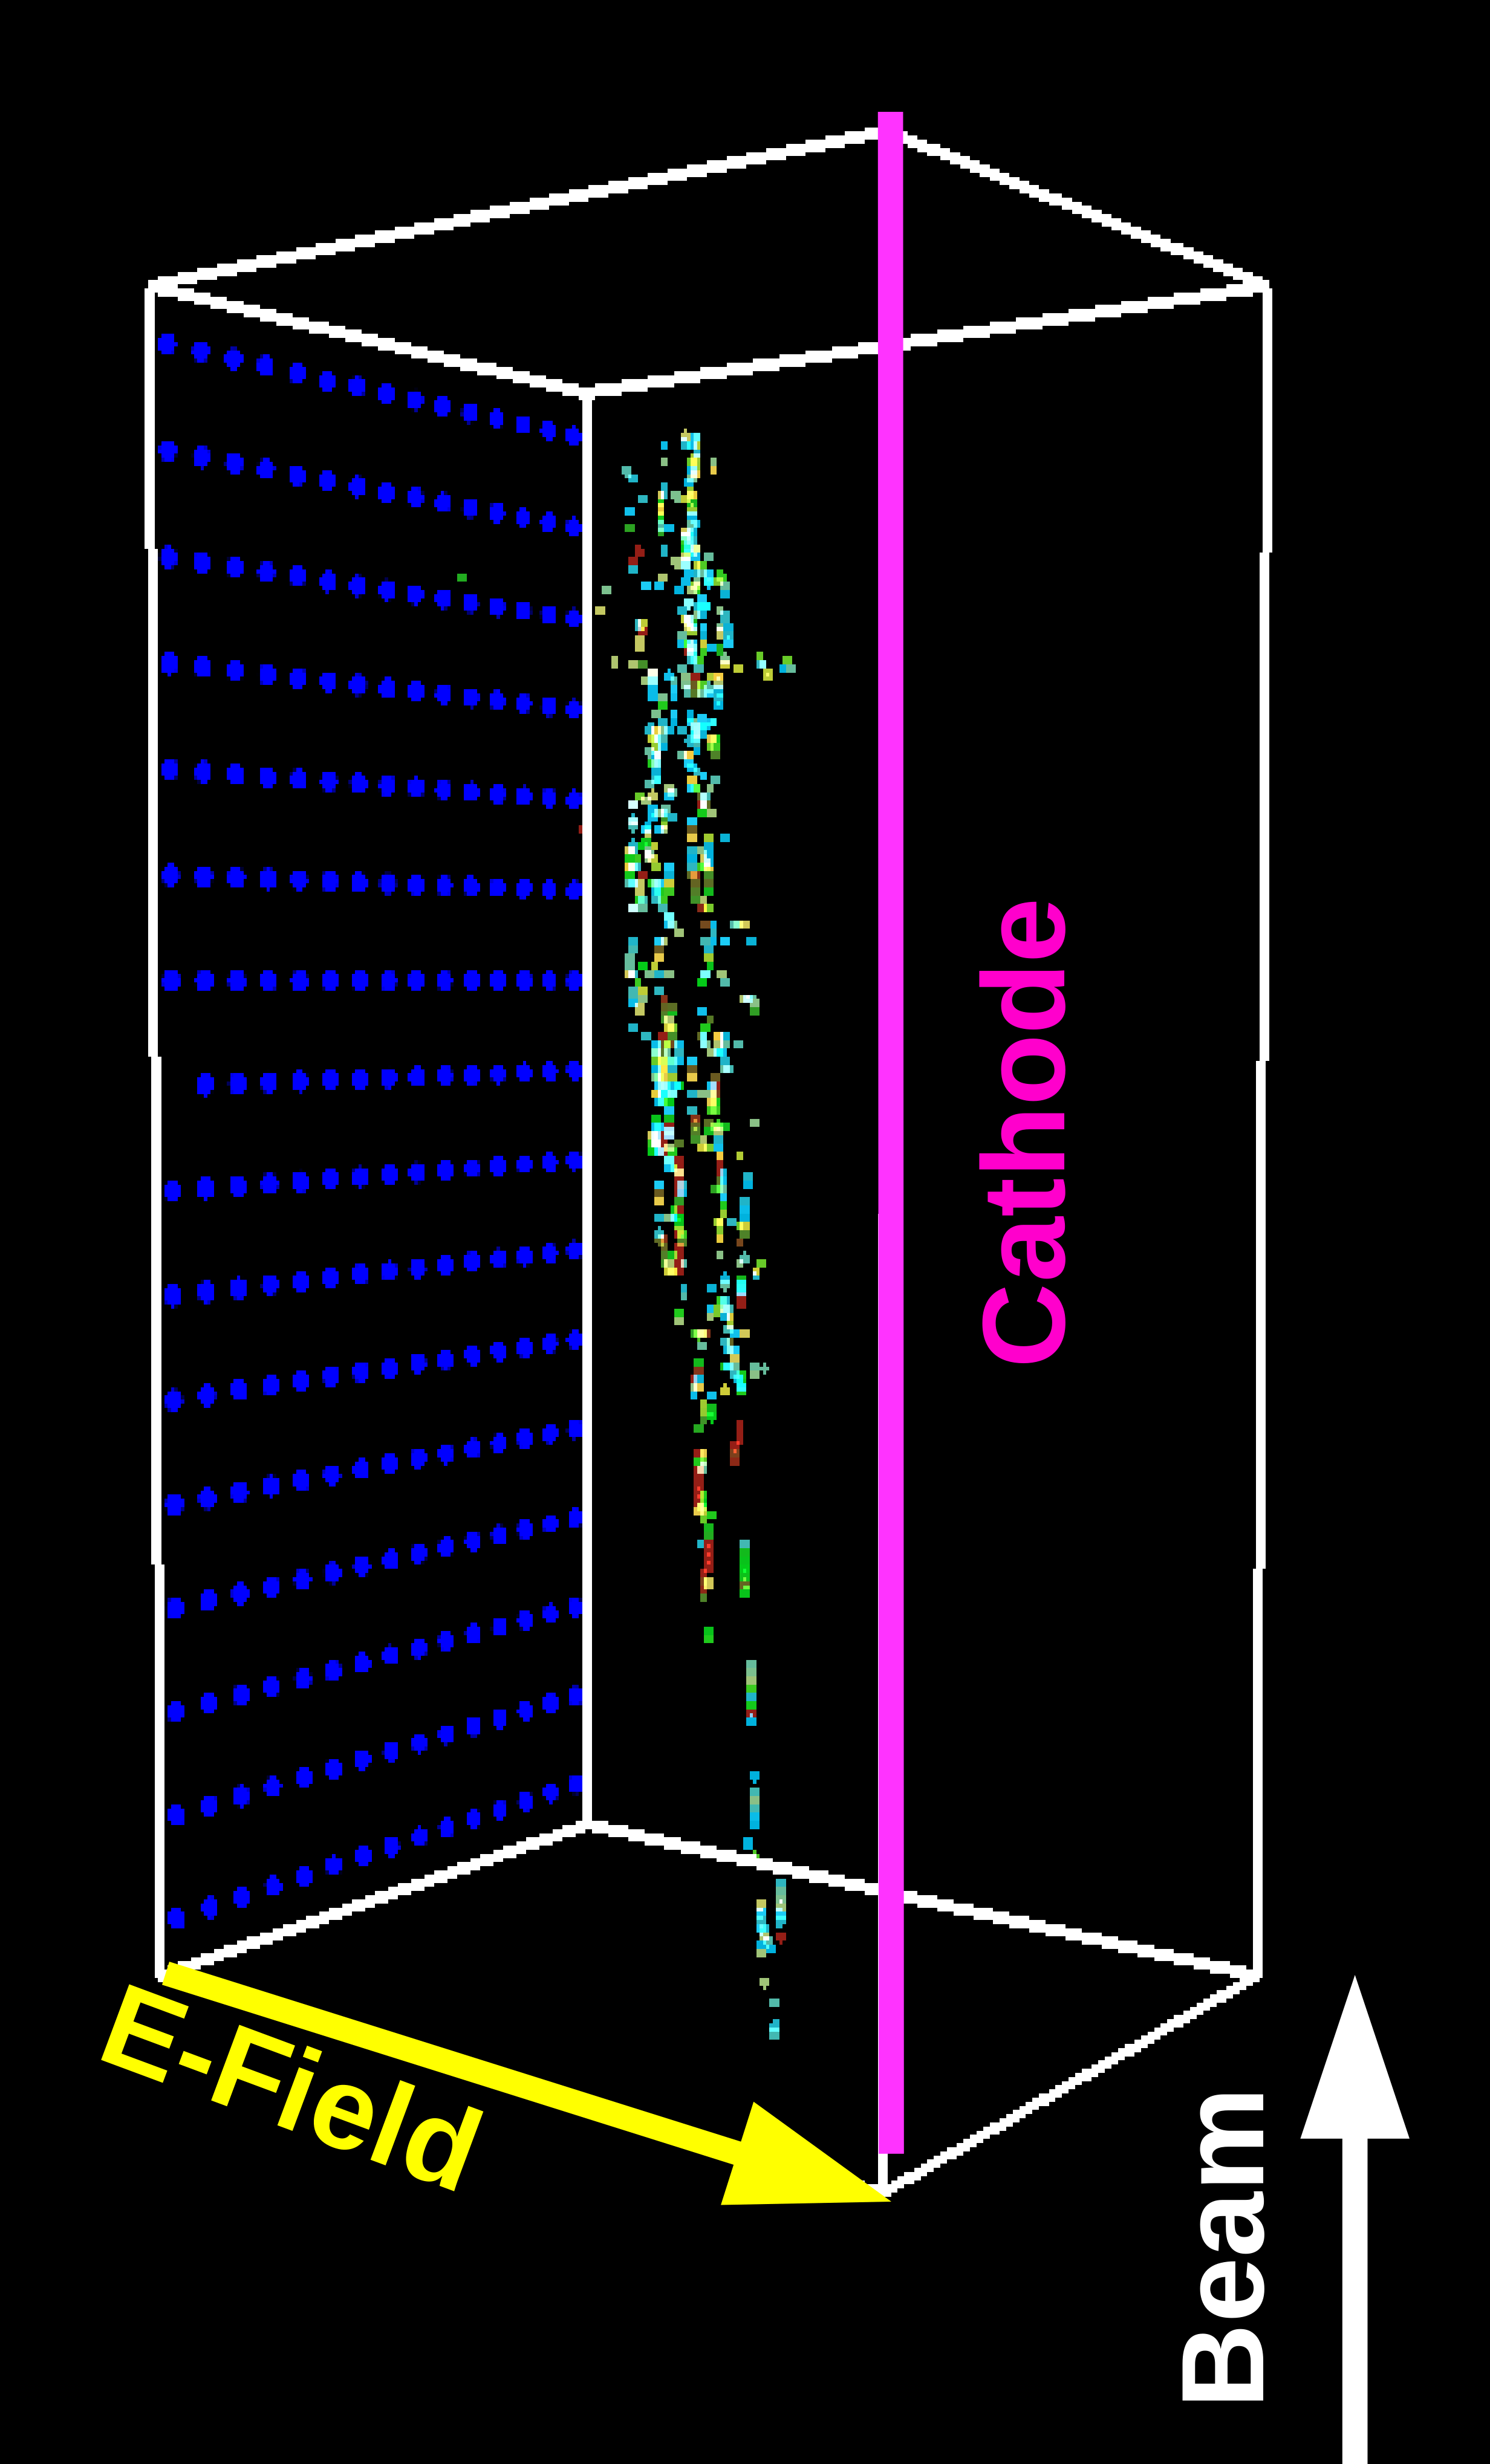
\includegraphics[width=.445\textwidth]{pixlar/pixlar_event_side}
	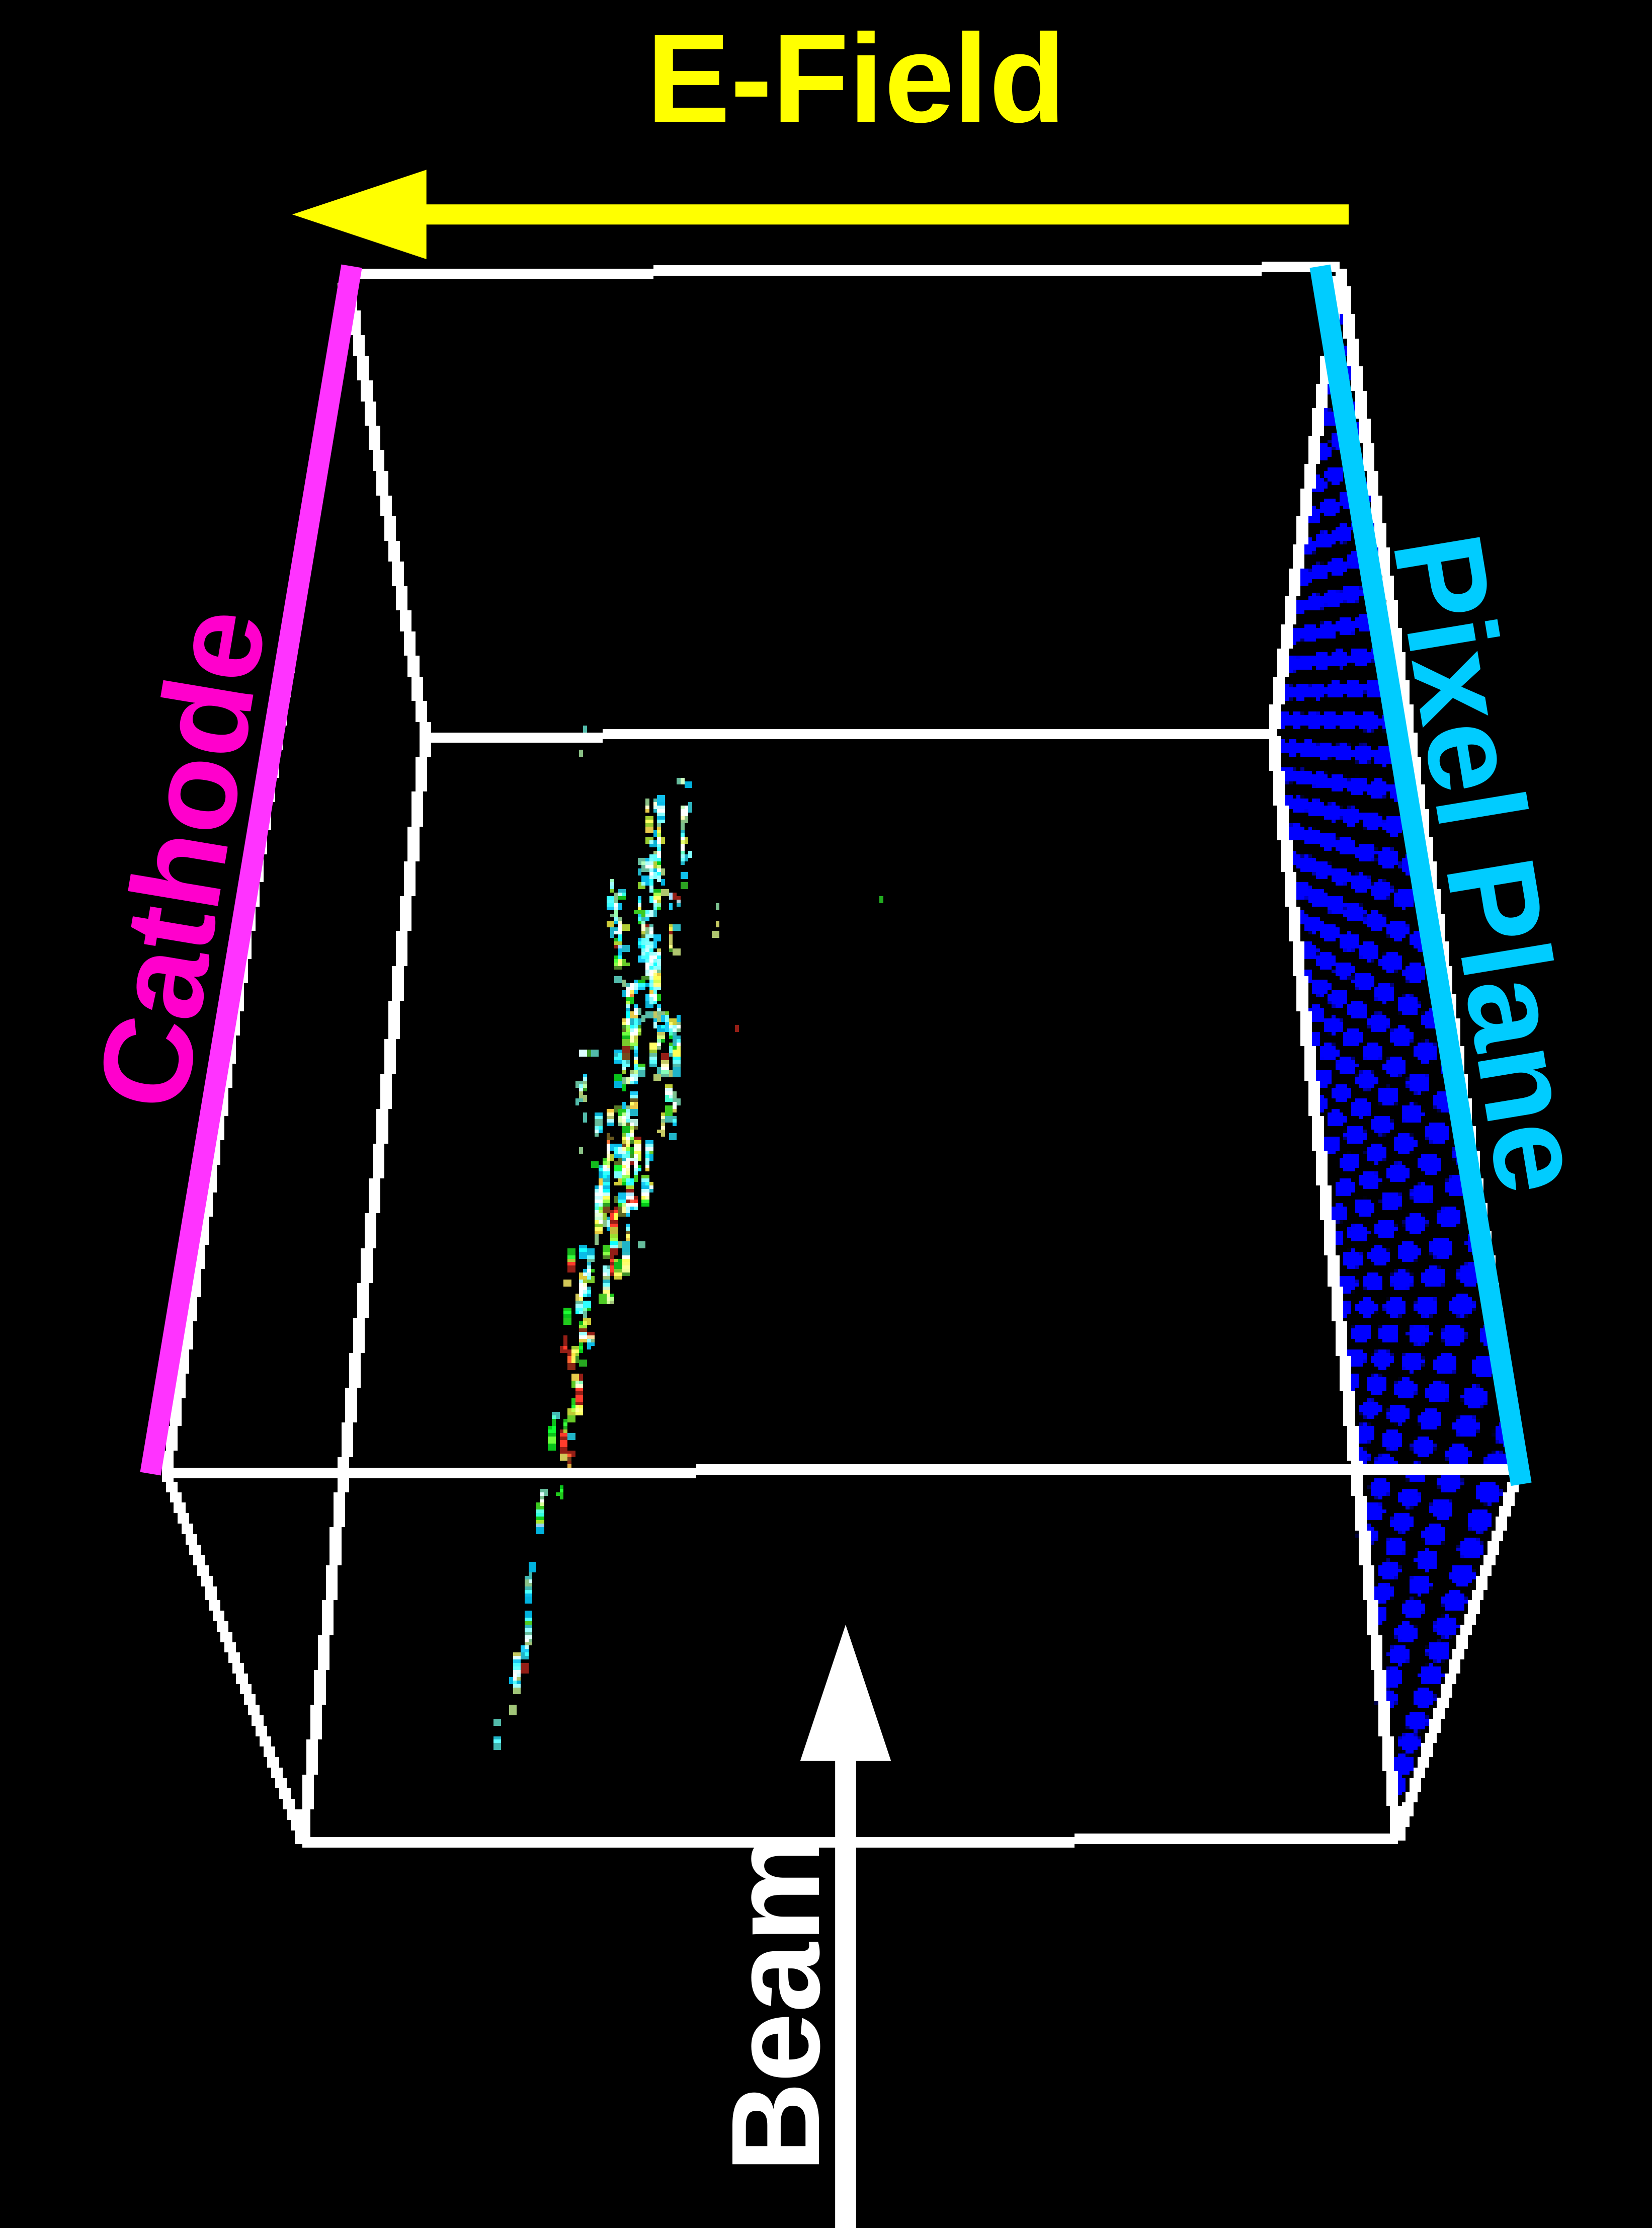
\includegraphics[width=.545\textwidth]{pixlar/pixlar_event_top}
	\caption{\pixlar{} beam event.}
	\label{fig:pixlar_event}
\end{figure}

Over several weeks, beam and cosmic muon data was taken.
At the time of this writing, no official results were available.
Nevertheless, preliminary analyses indicate a successful scale-up of the pixelated \lartpc{} concept.
The achieved \gls{snr} seems to be comparable to what was reached with the prototype at \gls{help} described above.
A recorded beam event is depicted in Figure~\ref{fig:pixlar_event}.